\documentclass[a4paper,11pt,BCOR=8mm,twoside,headsepline]{scrbook}
\author{Daniel Süß}
\title{Stochastic Dynamics of Open Quantum Systems}

% Basic input and font encoding
%\usepackage{scrhack}
\usepackage[utf8]{inputenc}
\usepackage[T1]{fontenc}
\usepackage[ngerman, english]{babel}

% math stuff
\usepackage{amsfonts, amsmath, amssymb, amsthm}

% pictures n stuff
\usepackage{graphicx}
\DeclareGraphicsExtensions{.pdf}
\usepackage{subcaption}
% labels for subfigures are capital
\renewcommand{\thesubfigure}{\Alph{subfigure}}

\usepackage{cite}
\usepackage{enumerate}

% tables
\usepackage{tabu}
\usepackage{multicol}


\usepackage{pgf}
\usepackage{tikz}
\usetikzlibrary{matrix}
\usetikzlibrary{calc}
\usetikzlibrary{arrows}
%\usetikzlibrary{external}
%\tikzexternalize[prefix=tikz/]

\usepackage{standalone}

% package to provide if-statements in new commands
\usepackage{ifthen}

% Correct spacing of abbreviations
\usepackage{xspace}

% enables referencing and generation of hyperlinks
\usepackage{hyperref}
\usepackage[all]{hypcap}

% some custom spacing
\usepackage{setspace}
\onehalfspacing
\usepackage[margin=0.8cm, font=small, labelfont=bf]{caption}

% better looking font setting
%\usepackage{microtype}

%\newcommand{\includetikz}[1]{%
%    \tikzsetnextfilename{#1}%
%    \input{img/#1.tikz}%
%}

%%%%%%%%%%%%%%%%%%%%%%%%%%%%%%%%%%%%%%%%%%%%%%%%%%%%%%%%%%%%%%%%%%%%%%%%%%%%%%%
% Custom commands

% Text commands/symbols
\newcommand{\idef}[1]{\emph{#1}}       % (i)nline (def)inition
\newcommand{\quotes}[1]{``#1''}
\newcommand{\nth}[1]{\textsuperscript{#1}\,}
\renewcommand{\th}{\nth{th}}
\newcommand{\cm}[1]{{\color{red}#1}}   % (c)orrection (m)ark
\newcommand{\NMSSE}{\textsc{NMSSE}\xspace}
\newcommand{\HEOM}{\textsc{HEOM}\xspace}
\newcommand{\ucm}{\mathrm{cm}}

% Math Macros
\newcommand{\cc}[1]{{#1}^*}
\newcommand{\abs}[1]{\vert #1 \vert}
\newcommand{\norm}[1]{\left\Vert #1 \right\Vert}
\newcommand{\op}[1]{#1}
\newcommand{\adj}[1]{\op{#1}^\dagger}
\newcommand{\dual}[1]{{#1}^*}

\newcommand{\E}[1][\empty]{%
  \ifthenelse{\equal{#1}{\empty}}
    {\mathbb{E}}
    {\mathbb{E}\left( #1 \right)}
}
\newcommand{\qmean}[1]{\langle #1 \rangle}

\renewcommand{\exp}[1][\empty]{%
  \ifthenelse{\equal{#1}{\empty}}
    {\mathrm{exp}}
    {\mathrm{e}^{#1}}
}
\newcommand{\Texp}[1][\empty]{%
  \ifthenelse{\equal{#1}{\empty}}
    {\operatorname{T}_+\mathrm{exp}}
    {\operatorname{T}_+\mathrm{e}^{#1}}
}
\newcommand{\varf}[1][\empty]{%
  \ifthenelse{\equal{#1}{\empty}}
    {\mathbb{\mathcal{C}}}
    {\mathcal{C}\left( #1 \right)}
}
\newcommand{\intl}[3]{\int_{#1}^{#2}\mathrm{d}#3\,}

\let\rvec\vec
\renewcommand{\vec}[1]{\boldsymbol{#1}}
\newcommand{\bra}[1]{\langle #1 |}
\newcommand{\ket}[1]{| #1 \rangle}
%\newcommand{\braket}[2]{\left\langle #1 \middle| #2 \right\rangle}
\newcommand{\braket}[2]{\langle #1 | #2 \rangle}
\renewcommand{\sp}[2]{\left\langle #1 , #2 \right\rangle}
\newcommand{\dualp}[2]{\left( #1 , #2 \right)}

\newcommand{\twovec}[2]{%
  \begin{pmatrix}
    #1 \\ #2
  \end{pmatrix}
}

% Math Symbols
\newcommand{\ii}{\mathrm{i}}
\newcommand{\dd}{\, \mathrm{d}}
\newcommand{\intdd}{\int\mathrm{d}}
%\newcommand{\Tr}[1]{\operatorname{Tr}_\mathrm{#1}}
\newcommand{\Tr}{\operatorname{Tr}}
\newcommand{\Res}{\operatorname{Res}}
\newcommand{\mudz}{\, \mu(\mathrm{d} z)}

\newcommand{\ZZ}{\cc{Z}}               % Our noise process
\newcommand{\tildeZZ}{\cc{\tilde Z}}
\newcommand{\adjZZ}{\mathcal{D}}         % and it's adjoint

\newcommand{\kk}{\vec{k}}
\newcommand{\zz}{\vec{z}}
\newcommand{\ww}{\vec{w}}
\newcommand{\qq}{\vec{q}}
\newcommand{\QQ}{\vec{Q}}

\newcommand{\psit}[1][\empty]{%
  \ifthenelse{\equal{#1}{\empty}}
    {\psi_t}
    {\psi_t^{(#1)}}
}
\newcommand{\psitz}[1][\empty]{%
  \ifthenelse{\equal{#1}{\empty}}
    {\psi_t(\cc\zz)}
    {\psi_t^{(#1)(\cc\zz)}}
}
\newcommand{\psitZ}[1][\empty]{%
  \ifthenelse{\equal{#1}{\empty}}
    {\psi_t(\ZZ)}
    {\psi_t^{(#1)}(\ZZ)}
}
\newcommand{\psitphi}{\psi_t(\cc{\vec\phi}_t(\cc\zz))}
\newcommand{\psio}[1]{\psi^{(#1)}}

\newcommand{\phitla}{\phi_{t, \lambda}}
\newcommand{\ccphitla}{\cc\phi_{t, \lambda}}

\newcommand{\ee}{\vec{e}}
\newcommand{\unit}{\op{\mathrm{I}}}    % Idendity operator/matrix
\newcommand{\PM}{\mathbb{P}}           % Probability measure
\newcommand{\ft}[1]{\Hat{#1}}
\newcommand{\ift}[1]{\check{#1}}
\newcommand{\CHF}{\mathcal{F}}         % Characteristic functional
\renewcommand{\propto}{\sim}

% Operators
\newcommand{\Htot}{H_\mathrm{tot}}
\newcommand{\Hsys}{H}
\newcommand{\Henv}{H_\mathrm{env}}
\newcommand{\Hint}{H_\mathrm{int}}
\newcommand{\opH}[1]{H_\mathrm{#1}}
\newcommand{\opT}[1]{T_\mathrm{#1}}
\newcommand{\opV}[1]{V_\mathrm{#1}}
\newcommand{\opU}[1]{U_\mathrm{#1}}

% Math Sets
\newcommand{\Complex}{\mathbb{C}}
\newcommand{\Reals}{\mathbb{R}}
\newcommand{\Integers}{\mathbb{Z}}
\newcommand{\SchwartzS}{\mathcal{S}}
\newcommand{\SchwartzSC}{\SchwartzS_\Complex}
\newcommand{\HH}{\mathcal{H}}
\newcommand{\HHenv}{\HH_\mathrm{env}}
\newcommand{\HHsys}{\HH_\mathrm{sys}}

% Environments
\newtheorem{thm}{Theorem}
\newtheorem{lem}[thm]{Lemma}
\theoremstyle{remark}
\newtheorem*{rem}{Remark}

% Make sure autoref print (.) for equations
\let\oldtheequation\theequation
\makeatletter
  \def\tagform@#1{\maketag@@@{\ignorespaces#1\unskip\@@italiccorr}}
  \renewcommand{\theequation}{(\oldtheequation)}
\makeatother

% Autoref commands
% \Autoref is for the beginning of the sentence
\let\orgautoref\autoref
\providecommand{\Autoref}
        {\def\equationautorefname{Equation}%
         \def\figureautorefname{Figure}%
         \def\subfigureautorefname{Figure}%
         \def\chapterautorefname{Chapter}
         \def\sectionautorefname{Section}%
         \def\subsectionautorefname{Section}%
         \def\subsubsectionautorefname{Section}%
         \def\Itemautorefname{Item}%
         \def\tableautorefname{Table}%
         \orgautoref}

% \Autorefs is plural for the beginning of the sentence
\providecommand{\Autorefs}
        {\def\equationautorefname{Equations}%
         \def\figureautorefname{Figures}%
         \def\subfigureautorefname{Figures}%
         \def\chapterautorefname{Chapters}
         \def\sectionautorefname{Sections}%
         \def\subsectionautorefname{Sections}%
         \def\subsubsectionautorefname{Sections}%
         \def\Itemautorefname{Items}%
         \def\tableautorefname{Tables}%
         \orgautoref}

% \autoref is used inside a sentence
% (this is a renew of the standard)
\renewcommand{\autoref}
        {\def\equationautorefname{Eq.}%
         \def\figureautorefname{Fig.}%
         \def\subfigureautorefname{Fig.}%
         \def\chapterautorefname{Chap.}
         \def\sectionautorefname{Sect.}%
         \def\subsectionautorefname{Sect.}%
         \def\subsubsectionautorefname{Sect.}%
         \def\Itemautorefname{item}%
         \def\tableautorefname{Table}%
         \orgautoref}

% \autorefs is plural for inside a sentence
\providecommand{\autorefs}
        {\def\equationautorefname{Eqs.}%
         \def\figureautorefname{Figs.}%
         \def\subfigureautorefname{Figs.}%
         \def\chapterautorefname{Chaps.}
         \def\sectionautorefname{Sects.}%
         \def\subsectionautorefname{Sects.}%
         \def\subsubsectionautorefname{Sects.}%
         \def\Itemautorefname{items}%
         \def\tableautorefname{Tables}%
         \orgautoref}


% centered table header
 \newcommand{\theader}[1]{\multicolumn{1}{c}{#1}}
\clubpenalty10000
\widowpenalty10000
\displaywidowpenalty=10000
%%%%%%%%%%%%%%%%%%%%%%%%%%%%%%%%%%%%%%%%%%%%%%%%%%%%%%%%%%%%%%%%%%%%%%%%%%%%%%%
%%%%%%%%%%%%%%%%%%%%%%%%%%%%%%%%%%%%%%%%%%%%%%%%%%%%%%%%%%%%%%%%%%%%%%%%%%%%%%%
%\includeonly{introduction}
%\includeonly{nmqsd,appendix}
%\includeonly{numerics}
%\includeonly{application}
%\includeonly{conclusions}

\begin{document}
\frontmatter
%%%%%%%%%%%%%%%%%%%%%%%%%%%%%%%%%%%%%%%%%%%%%%%%%%%%%%%%%%%%%%%%%%%%%%%%%%%%
% Title Page
\thispagestyle{empty}
\vspace{-5em}
\begin{flushleft}
  
\includegraphics[angle=0,width=60mm]{img/TU_Logo_SW.pdf}
  \par
\end{flushleft}
\vspace{-3em}
\begin{center}\rule{\textwidth}{0.1ex}\par\end{center}
\vspace{-4em}
\begin{center}\rule{\textwidth}{0.1ex}\par\end{center}

\vfill
\begin{center}\textbf{\Huge Stochastical Dynamics of}\par\end{center}
\begin{center}\textbf{\Huge Open Quantum Systems}\par\end{center}
\vfill
\begin{center}
{\large Diplomarbeit}\\
{\large zur Erlangung des wissenschaftlichen Grades}\\
{\large Diplom-Physiker}\par
\end{center}

\begin{center}vorgelegt von\par\end{center}
\begin{center}{\large Daniel Süß}\\geboren am 18.10.1987 in
Dresden\par
\end{center}
\vspace{13mm}
\begin{center}
{\large Institut für Theoretische Physik}\\
{\large der Technischen Universitaet Dresden}\\
{\large 2013}\par
\end{center}

%%%%%%%%%%%%%%%%%%%%%%%%%%%%%%%%%%%%%%%%%%%%%%%%%%%%%%%%%%%%%%%%%%%%%%%%%%%%%
% Referee Pages
\newpage
\thispagestyle{empty}
\ \vfill
\begin{tabular}{l}
%Eingereicht am ???\\
\end{tabular}

\vspace{1cm}

\begin{tabular}{ll}
1.~Gutachter: & Herr Prof. Dr. Walter T. Strunz\\
%2.~Gutachter: & Herr Prof. Dr. ???\\
\end{tabular}

%%%%%%%%%%%%%%%%%%%%%%%%%%%%%%%%%%%%%%%%%%%%%%%%%%%%%%%%%%%%%%%%%%%%%%%%%%%%%
% Abstract
\newpage
\thispagestyle{empty}
\section*{\centering{Zusammenfassung}}
\section*{\centering{Abstract}}
%%%%%%%%%%%%%%%%%%%%%%%%%%%%%%%%%%%%%%%%%%%%%%%%%%%%%%%%%%%%%%%%%%%%%%%%%%%%%
\tableofcontents
%%%%%%%%%%%%%%%%%%%%%%%%%%%%%%%%%%%%%%%%%%%%%%%%%%%%%%%%%%%%%%%%%%%%%%%%%%%%%

\mainmatter
\newpage

\chapter{Introduction}
\label{chap:introduction}
% * Classical/Quantum closed time evolution
% * necessity for open systems

% Quantum mechanics, hydrogen, larger system
% hydrogen in external field, classical environment
% open system viewpoint, simplest kind of environment: measurement
%  * exchange of energy, momentum, angular momentum, phase, charge, ...
%  * Schrödinger equation: closed system; appromation
%  * bath degrees of freedom uninteresting!
%  * best cut: system = all degrees of freedom relevant to describe experiment
%  * examples

The explanation of the discrete Hydrogen-spectrum in terms of Matrix-mechanics by Heisenberg and Wave-mechanics by Schrödinger is often perceived as the hour of birth for modern quantum theory.
Since then, the desire to understand systems with an increasing number of degrees of freedom and ever-growing complexity has been a main driving force behind the development of new theoretical ideas.
However, the overwhelming majority of quantum mechanical insights relies on more or less severe approximations, as even apparently simple models like the Helium atom have not been solved analytically.
One simplification that underlies all physical investigation is the distinction between relevant and irrelevant degrees of freedom for a certain situation:
Even the simple Hydrogen model, made up from an electron-proton pair and the mutual Coulomb attraction, ignores the surrounding electrons and protons in the same container, to give an example.
While under many circumstances the relevant degrees of freedom behave like an isolated unit, there are examples where environmental effects significantly shape the dynamical behavior of the system under consideration---these are referred to as open quantum systems.
Clearly, the cut distinguishing between relevant system and irrelevant environment is not uniquely defined, but generally, the requirement to account for a given experimental setting eliminates ambiguities to the greatest possible extent.

% Open Classical System
% * possibly only true closed system: universe
% * classical open systems
% * Brownian motion
% * colission based models
% * well understood, friction and fluctuations, but not conceptual that much harder
%  * still well defined system state
% * QM ENTAAAAANGLEMENT!!!!

Of course, the previous discussion applies not only to quantum mechanics:
A closed classical system is described by phase space coordinates $(p,q)$ and canonical equations of motion in the Hamiltonian framework.
To account for the influence of an environment, the latter are simply extended by fluctuation- and friction-forces leading to an irreversible time evolution governed by the stochastic Langevin equation \cite{GaCr85_handbook}.
A different description arises by averaging trajectories corresponding to different noise-realizations, the resulting probability density on phase space satisfies the Fokker-Planck equation.
However, both points of view are completely equivalent; there is no conceptual problem in assigning a pure state, namely a phase space point $(p(t),q(t))$, to a given trajectory at any time $t$---this simplifies matters dramatically compared to an open quantum system.

%%%%%%%%%%%%%%%%%%%%%%%%%%%%%%%%%%%%%%%%%%%%%%%%%%%%%%%%%%%%%%%%%%%%%%%%%%%%%%%
\section{Open Quantum Systems}
\label{sec:intro.open_quantum}
% * feynman-vernon
% * projection operator
% * markovian stochastic schrödinger equations
% * markov vs nonmarkov
% * Measure of non-Markovianity
% * Why SSE? --> ρ always positive -->
% * quapi
% * Connection to linear response theory Weiss Ch. 6
%%%%%%%%%%%%%%%%%%%%%%%%%%%%%%%%%%%%%%%%%%%%%%%%%%%%%%%%%%%%%%%%%%%%%%%%%%%%%%%

% general open system
%  * product Hilbert space (or one isomorphic)
%  * reduced density matrix; all answers
%  * although complete state pure; entanglement causes mixed reduced state

In order to determine the dynamics of an open quantum system from first principles, we proceed as follows:
First we embed the system into an environment such that both combined can be regarded as a closed system for all practical matters.
Mathematically, the kinematic structure is given by the product $\HHsys\otimes\HHenv$ or any Hilbert space isomorphic to it.
For such an isolated system, the time evolution is governed by the usual postulates of quantum mechanics, that is the Schrödinger or the von Neumann equation for pure or mixed initial state, respectively.
Since the environment's purpose is merely to restore a unitary time evolution, all relevant information about the system is encoded in the \emph{reduced state} $\rho(t) = \Tr_\mathrm{env} \rho_\mathrm{tot}(t)$ obtained by tracing over the environmental degrees of freedom.
Formally, this amounts to assigning the expectation value
\begin{equation}
  \qmean{A} := \Tr(\rho_\mathrm{tot}(t) \, A\otimes I_\mathrm{env}) = \Tr_\mathrm{sys}(\rho(t) \, A)
  \label{eq:intro.reduced_state}
\end{equation}
to each observable $A$ on $\HHsys$.
The second part, namely that $\qmean{\cdot}$ defines a genuine trace-class operator $\rho_t$ on $\HHsys$, follows under some additional regularity assumptions \cite{BrRo03_operator_algebras}.
Although the total system-bath state is pure at any given time, the reduced state is not necessarily a pure-state projector.
On the contrary, quantum entanglement caused by the interaction requires assigning a true mixture to the system---this makes the treatment of open quantum system so much harder compared to its classical counterpart.\\



% Two approaches: embedding into larger/axiomatic, why we choose later
% master equations
%  * trace out degrees of freedom (microscopical)
%     * only approximately, phenomonological models (redfield)
%        * valid only for some initial conditions
%        * possibly unphyical behavior due to purely perturbational treatment (Breuer or Cohen-Tanduij)

Although the reduced state's time evolution is uniquely defined by the von Neumann equation for $\rho_\mathrm{tot}(t)$ and \autoref{eq:intro.reduced_state}, a dynamical equation purely in terms of $\rho(t)$, a \emph{Master equation}, is more desirable for all practical purposes.
In general, the derivation of a closed equation in $\rho(t)$ from the unitary system-bath evolution relies on quite severe approximations.
A typical example is the \emph{Redfield}-equation \cite{BrPe2002_open_quantum}, which is based on the following physical assumptions:
First, one starts with a initial product state $\rho_\mathrm{tot}(0) = \rho(0) \otimes \rho_\mathrm{env}$.
By the weak-coupling or \emph{Born}-approximation, this product form with a fixed environmental state $\rho_\mathrm{env}$ is preserved for all times.
Furthermore, we assume that the dynamics of the environment proceed on a much smaller timescale compared to the system and any \quotes{memory}-effects are negligible small---this is the \emph{Markov}-approximation
However, because it is derived from a truncated perturbation expansion, the Redfield-master equation does not necessarily preserve all properties of a genuine density matrix.

%  * Linblad: (axiomatic)
%     * Born Approx: weak coupling, incluence of system on env. small
%     * Markov: memory
%       => semi-group; timescales
%     * quantum dynamics semi-group additionally completely positive
%        * general form: Linblad (at least for finite system)
% Markov approx well founded in quantum optics (high transition frequencies, weak coupling, short correlation time)
%     * operator algebras

A more robust approach based on similar physical assumptions, but more axiomatic in spirit has been elaborated by Linblad \cite{Li76_generators_qdsg}:
It is formulated purely in terms of propagators $\Lambda_t$ on the system's Hilbert space without making reference to a certain environment.
The Born-Markov approximation is rephrased to the condition that the family of maps $(\Lambda_t)_{t\ge 0}$ constitute a quantum dynamical semi-group \cite{AlLe87_qds}, namely $\Lambda_{s+t} = \Lambda_s\Lambda_t$.
Provided the $\Lambda_t$ are completely-positive as well, the corresponding Master equation for the reduced state necessarily takes the Linblad form
\begin{equation}
  \partial_t \rho_t = - \frac{\ii}{\hbar} [H, \rho_t] + \frac{1}{2}\sum_n \left( [L_n\,\rho_t, \adj{L}_n] + [L_n, \rho_t\,\adj{L}_n] \right).
  \label{eq:intro.linblad}
\end{equation}
Here $H = \adj{H}$ is a self-adjoint operator and $L_n$ are Linbladians describing various irreversible channels \cite{WiMi10_measurement}.

% Nowadays: Non-Markovian effects
%  * examples:
%     * solid state physics: tunneling qubit?
%     * quantum optics: decay into structued environment; cavity gedöhns, photonic band gap materials
%     * chemical- and biological systems:
%  * general problems: no general master equation
%  * Najma zwanzig projection operator --> systematic investigation
%     * approximation in practical evaluation: product initial state; although general case possible by ???
%     * unwieldy numerics due to memory effecs,

% TODO Add applications...
no universally valid and tractable non-Markovian generalization of the Lindblad Master equation is known today.
The projection formalism of Nakajima-Zwanzig provides a closed equation in the reduced state $\rho_t$ by separating relevant and irrelevant degrees of freedom in the von Neumann equation \cite{BrPe2002_open_quantum}.
However, it includes non-Markovian effects by a memory-integral such that the evolution of $\rho(t)$ depends on all reduced states at times prior to $t$.
This renders analytical or numerical solutions without further approximations virtually impossible.\\

% Alternative: Feynman Vernon
%  * direct calculation of path integrals
%  * problematic due to oscillatory effecs
%  * equivalent, but more better suited: Tanimura hierarchy

A completely different approach to the dynamics of open quantum systems is the influence-functional formalism \cite{FeVe63_quantum_dissipative,FeHi10_path_integrals}:
Besides its strength in analytical calculations


%%%%%%%%%%%%%%%%%%%%%%%%%%%%%%%%%%%%%%%%%%%%%%%%%%%%%%%%%%%%%%%%%%%%%%%%%%%%%%%%
\section{Unravellings}
\label{sec:intro.unravellings}

% Classical Mechanics: equivalance between Fokker-Planck
%  * evolution of probability density function of finite dim. cont. Markov process
% and Langevin equation: Stochastic DE, "process realizations"
% => Connection between partial differential equations and stochastic processes: Feynman Kac Formula
%  * lies at the Heart of the Path integral formulation



% Quantum mechanics: Markovian regime
%  * Stochastic Schrödinger equation for pure states
%  * such that average coincides with reduced density operator
% diffusive equation (linear and nonlinear)
% jump unravellings
% favored due to smaller size, parallelization, always positive density operator\cite{GaWi02_real_nmsse}
% Monte-Carlo: Take E(...) and evaluate for "random" trajectories; N-->\infty should work fine by law of large numbers
% favored, since they contain more information; we have a pure product state for open system!!; still have environmental degrees of freedom
%


% NMSSE
%  * based on microscopical model, not unravelling
%  * without any approximations
%  * encodes all information in bcf (similar to Dissipation-Fluctuation Theorem)
%  * good for studying transition to Markov; but also by assuming (possibly unphyical) bcf numerical investigation!!!
%  * can provide master equation
% Also fermionic environment



% Alternative Non-Markovian Description:
%  * Jump equations (Jack)
%  * Pseudo-Modes (used for spectra):
%     * for bcf used in this work, possible to replace Non-Markovian env. by damped oscillators coupled to Markovian bath
%     => usual trajectoriy treatment



%%%%%%%%%%%%%%%%%%%%%%%%%%%%%%%%%%%%%%%%%%%%%%%%%%%%%%%%%%%%%%%%%%%%%%%%%%%%%%%
\section{Established Results and Subject of this Work}
\label{sec:into.results}
% * Collission models
% * Tanimura Hierarchies
% * NMQSD (also for fermionic)
% * results
%%%%%%%%%%%%%%%%%%%%%%%%%%%%%%%%%%%%%%%%%%%%%%%%%%%%%%%%%%%%%%%%%%%%%%%%%%%%%%%

% We want to solve NMSSE!!!
%
% * Analytical solutions
% TODO ZOFE and functional expansion of O operator
%  * spectra and transfer in ...
% All based on a uncontrolled assumption of O operator

% Here we try to do it without; closely related to Tanimura
% Hierarchy linear and nonlinear


%%%%%%%%%%%%%%%%%%%%%%%%%%%%%%%%%%%%%%%%%%%%%%%%%%%%%%%%%%%%%%%%%%%%%%%%%%%%%%%
\section{Outline}
\label{sec:into.outline}
%%%%%%%%%%%%%%%%%%%%%%%%%%%%%%%%%%%%%%%%%%%%%%%%%%%%%%%%%%%%%%%%%%%%%%%%%%%%%%%


\chapter{Non-Markovian Quantum State Diffusion}
\label{chap:nmqsd}
% * lin/nonlin Markovian SSE
% * little History
% * alternatives standard (projection?), pseudomodes
% * relevant/irre



%%%%%%%%%%%%%%%%%%%%%%%%%%%%%%%%%%%%%%%%%%%%%%%%%%%%%%%%%%%%%%%%%%%%%%%%%%%%%%%
\section{The Microscopical Model}
\label{sec:nmqsd.model}
% * standard model (why oscillators, why linear coupling?)
% * reservoir/environment
% * initial states
%
% TODO Begin more positive!
% TODO elaborate on why we choose linear coupling
% TODO Nonlinear models?
% TODO initial state; correlation function
% TODO Typical correlation functions for infinite systems; decay rate, etc.
% TODO Why oscillator bath?! Feynman Hibbs p.354 --> all cold baths are equivalent
% TODO This correlation function only T=0, general see Weiss (6.11)
%%%%%%%%%%%%%%%%%%%%%%%%%%%%%%%%%%%%%%%%%%%%%%%%%%%%%%%%%%%%%%%%%%%%%%%%%%%%%%%

Although the first and foremost goal of our work is the description of the system's reduced dynamics, we focus on a full system-environment description at first.
On one hand this serves the purpose to better understand the emergence of the typical phenomena when dealing with open quantum systems and their dependence on the bath.
But more important, starting with a closed quantum system is the only strategy that enables a derivation from first principles, in our case the Schrödinger equation.
A last argument in favor of the microscopic approach, PRODUCT STATES, ENTANGLEMENT, etc. ---we will not dwell on the this any further.\\

As a starting point we consider an environment consisting of a finite number $N$ of uncoupled harmonic oscillators.
%\footnote{We will use "environment", "reservoir" and "bath" interchangeably, altough the later two suggest a large size compared to the system.}
This model has been studied extensively for example in the book of Weiss \cite{We99_dissipative_systems}.
The generalization to an infinite number can be carried out formally along the same lines, replacing sums by infinite series or even integrals; a different approach within our framework is presented later.
The dynamics of both the system and the environment are then described by a unitary time evolution governed by the Hamiltonian
\begin{equation}
  \Htot = \Hsys \otimes \unit  +  \unit \otimes \Henv  +  \Hint,
  \label{eq:nmqsd.Htot}
\end{equation}
where $\Hsys$ and $\Henv$ are the free Hamiltonians of the system and the bath respectively.\footnote{For some models like the damped harmonic oscillator \cite{CaLe83_diss_system} an additional renormalization term arises from the interaction. Nevertheless such a contribution is best attributed to $\Hsys$ since it only acts on the system's Hilbert space.}
The later is a sum over independent harmonic oscillators $\Henv = \sum_\lambda \omega_\lambda \adj{a}_\lambda a_\lambda$ expressed in the ladder operators $a_\lambda$ and $\adj{a}_\lambda$ of the $\lambda$-th mode with frequency $\omega_\lambda$.
Treating a finite number of independent reservoirs poses no further difficulties and therefore is not elaborated in this section.

For the interaction between environment and system we confine ourselves to the case of linear coupling
\begin{equation}
  \Hint = \sum_\lambda \cc{g}_\lambda \, L \otimes \adj{a}_\lambda + g_\lambda \, \adj{L} \otimes a_\lambda.
  \label{eq:nmqsd.Hint}
\end{equation}
Here $L$ denotes the coupling operator in the system's Hilbert space and $g_\lambda \in \Complex$ the coupling strength of the $\lambda$-th mode.
Since in typical examples the coupling of an individual bath mode scales inversely with the environment size \cite{We99_dissipative_systems} the linear coupling in~\ref{eq:nmqsd.Hint} seems reasonable for macroscopic large environments.
%TODO stop repetition in "environment"
But our framework also incorporates small environments---even to the extreme of a single harmonic oscillator---with strong coupling as well.
For such cases the linearity needs to be seen as a further assumption of the model.

Beside the Hamiltonian the choice of initial conditions influences the system's subdynamics as well.
Throughout this work we only consider product initial conditions, where the bath is in the vacuum state with respect to all $a_\lambda$
\begin{equation}
  \ket{\Psi_0} = \ket{\psi_0} \bigotimes\limits_\lambda \ket{0_\lambda}.
  \label{eq:nmqsd.initial_conditions}
\end{equation}
These allow us to treat thermal bath states as we show in \autoref{sec:nmqsd.temperature}.\\

To absorb the free dynamics of the environment in time dependent creation and annihilation operators, we switch to the interaction picture with respect to $\Henv$.
Since the bath operators only obtain an additional phase $\exp[\pm \ii \omega_\lambda t]$, the transformed Hamiltonian from \autoref{eq:nmqsd.Htot} reads\footnote{We refrain from introducing another label to distinguish between time-evolution pictures---in what follows we always work in the interaction picture.}
\begin{equation}
  \Htot(t) = \Hsys \otimes \unit  +  \sum_\lambda \left( \cc{g}_\lambda \exp[\ii \omega_\lambda t] \, L \otimes \adj{a}_\lambda + g_\lambda \exp[-\ii \omega t] \, \adj{L} \otimes a_\lambda \right).
  \label{eq:nmqsd.Htot}
\end{equation}
Our choice of unentangled initial conditions with a thermal bath state ensures that the reduced density operator remains unaffected under the change of time-evolution picture.

%TODO This is just copied!
It is instructive to rewrite the last equation using the operator valued force
\begin{equation}
  B(t)=\sum_\lambda g_\lambda a_\lambda \exp[-\ii\omega_\lambda t].
  \label{eq:nmqsd.force_operator}
\end{equation}
The total Hamiltonian then reads $\Htot(t) = \Hsys \otimes \unit  +  L \otimes \adj{B(t)}  +  \adj{L} \otimes B(t)$.
Already from this equation it can be seen, that the complete action of the environment on the system is encoded in the operators $B(t)$.
%TODO Really?
In \autoref{sub:nmqsd.interpretation.time_osci} we introduce an explicit representation of these force operators and discuss their relation with the classical driving and friction forces.
An important---and within our model the only---characteristic of them is the correlation function
\begin{equation*}
  \alpha(t-s) = \big\langle  (B(t) + \adj{B(t)})(B(s) + \adj{B(s)}) \big\rangle_\rho,
\end{equation*}
where $\langle\cdot\rangle_\rho$ stands for the quantum average over the bath state $\rho$.
For a thermal state at temperature $T$, the correlation function can be calculated analytically \cite{FeHi10_path_integrals}
\begin{equation}
  \alpha_\beta(t - s) = \sum_\lambda  \vert g_\lambda \vert^2  \left( \operatorname{coth} \frac{\beta\omega_\lambda}{2} \, \cos \omega_\lambda (t-s)  -  \ii \sin \omega_\lambda(t-s) \right).
  \label{eq:nmqsd.thermal_correlation_function}
\end{equation}
In the limit of zero temperature and under the natural assumption that $\omega_\lambda > 0$, \Autoref{eq:nmqsd.thermal_correlation_function} goes over to
%TODO Add

%%%%%%%%%%%%%%%%%%%%%%%%%%%%%%%%%%%%%%%%%%%%%%%%%%%%%%%%%%%%%%%%%%%%%%%%%%%%%%%
\section{Linear NMSSE}
\label{sec:nmqsd.lin_nmsse}
% * Bargman States, hilbert space valued functions
% * derivation
% * problems, non-locality in noise
% * reduced density operator
% * relative state --> interpretation; but also connection with H_s valued functions
% * zero temperature, importance for calculations
% * quantum trajectory Carmichael
%
% TODO define \HHsys
% TODO Citations for full dynamics
% TODO Short proof for analyticity
% TODO Why we write \cc\zz always?
% TODO Proove of functional chain rule?
% TODO Citations of Strunz papers
% TODO stochastic <-> function are the same thing!
% TODO relation to unravelling
% TODO Good, since arbitary α --> infinite size system
%
%%%%%%%%%%%%%%%%%%%%%%%%%%%%%%%%%%%%%%%%%%%%%%%%%%%%%%%%%%%%%%%%%%%%%%%%%%%%%%%

The first step toward a solution of the full equations of motion~\ref{eq:???} for a realistic system is a reformulation first proposed by Diósi and Strunz\cite{DiSt97_nmsse}:
Expressing the bath degrees of freedom in the Segal-Bargmann Hilbert space of analytic functions\cite{Ba61_coherent_states,Se???} provides a representation that is well suited for a Monte-Carlo treatment.
To this end we introduce the unnormalized coherent state $\ket{z_\lambda} = \exp(z_\lambda \adj{a}_\lambda)\ket{0_\lambda}$ for each mode.
With the shorthand notation $\ket{\zz} = \bigotimes_\lambda \ket{z_\lambda}$, the resolution of the identity for the environment reads
\begin{equation}
  \unit = \int \frac{\exp[-\abs{\zz}^2]}{\pi^N} \, \ket{\zz}\bra{\zz} \dd^{2N}z,
  \label{eq:nmqsd.identity}
\end{equation}
where the integration measure is given by $\dd^{2N}z = \prod_\lambda \dd\Re z_\lambda \dd\Im z_\lambda$.
Throughout this work we often use the shorthand notation $\mudz = \pi^{-N} \exp(-\abs{\vec z}^2) \dd^{2N}z$, which turns out to be meaningful even for an uncountable number of bath oscillators.
\Autoref{eq:nmqsd.identity} allows us to express the full state in a time-independent environment basis
\begin{equation*}
  \ket{\Psi_t} = \int \ket{\psi_t(\cc\zz)} \otimes \ket{\zz} \mudz.
\end{equation*}
For the following derivation it is important to notice that the Segal-Bargmann transform $\zz \mapsto \psi_t(\cc\zz)$ is an anti-holomorphic, $\HHsys$ valued function.
It is equivalent to any other representation of the full state $\ket{\Psi_t}$.
Although the coherent states are not orthogonal, but rather satisfy $\braket{\vec w}{\vec z} = \exp(\sum_\lambda \cc w_\lambda z_\lambda)$, we can write for the reduced density matrix
%TODO Does this need a prove?
\begin{equation}
  \rho(t) = \Tr{env} \ket{\Psi_t}\bra{\Psi_t}
          = \int \ket{\psi_t(\cc\zz)}\bra{\psi_t(\cc\zz)} \mudz.
  \label{eq:nmqsd.reduced_matrix}
\end{equation}
After fixing the kinematic structure, the next step is to rewrite the dynamics: the representation of the ladder operators follow from the usual rules $\bra\zz \adj{a}_\lambda = \cc z_\lambda \bra\zz$ and $\bra\zz a_\lambda = \partial_{\cc z_\lambda} \bra\zz$\cite{???}.
These expressions give us the complete Schrödinger equation~\ref{eq:???} in the transformed space
\begin{equation}
  \partial_t \psi_t(\cc\zz) = -\ii\Hsys\psi_t(\cc\zz)  -  \ii L \sum_\lambda \cc g_\lambda \exp[-\ii\omega_\lambda t] \cc z_\lambda \, \psi_t(\cc\zz)  -  \ii \adj{L} \sum_\lambda g_\lambda \exp[\ii\omega_\lambda t] \, \frac{\partial \psi_t}{\partial z_\lambda}(\cc\zz).
  \label{eq:nmqsd.hamiltonian_microsopic}
\end{equation}
Introducing an effective driving process similar to \autoref{eq:nmqsd.force_operator}
\begin{equation}
  \ZZ_t(\cc\zz) = - \ii \sum_\lambda \cc g_\lambda \exp[\ii \omega_\lambda t] \cc z_\lambda
  \label{eq:nmqsd.stochastic_process}
\end{equation}
allows us to combine the effect of the first bath-interaction term into a single operator.
%TODO Proof?
A similar conversion works for the second term as well with the help of the functional chain rule $\frac{\partial}{\partial \cc z_\lambda} = \int \frac{\partial \ZZ_s}{\partial\cc z_\lambda} \frac{\delta}{\delta \ZZ_s} \dd s$.
our new equation of motion for the Segal-Bargmann transform reads
\begin{equation}
  \partial_t \psi_t = -\ii\Hsys\psi_t  +  L\ZZ_t\psi_t  -  \adj{L} \int_0^t \alpha(t-s) \frac{\delta \psi_t}{\delta \ZZ_s} \dd s.
  \label{eq:nmqsd.nmsse}
\end{equation}
As we shown in \autoref{sub:nmqsd.interpretation.unitary_view}, the integral boundaries arise due to the vacuum initial conditions~\ref{eq:nmqsd.initial_conditions}.
These render $\psi_0$ independent from the driving process, such that causality can be used to confine the integral domain.\\


Up to now we have always referred to \autoref{eq:nmqsd.nmsse} as a transformed Schrödinger equation in the full Hilbert space of both system and bath.
A different attitude is common as well: \Autoref{eq:nmqsd.reduced_matrix} can be rewritten as $\rho_t = \E[\ket{\psi_t}\bra{\psi_t}]$, where $\E\,\dots$ denotes the average over $\mudz = \pi^{-N} \exp(-\abs{\vec z}^2) \dd^{2N}z$.
Put differently the reduced density matrix $\rho_t$ arises as average over the stochastic pure state projectors $\ket{\psi_t(\zz)}\bra{\psi_t(\zz)}$.
Hence we regard \autoref{eq:nmqsd.nmsse} as a stochastic differential equation for the realisation $\psi_t(\zz)$.
We refer to the later either as system state relative to $\ket{\zz}$ or, in the spirit of the stochastic Schrödinger equations emerging from continuous measurements \cite{Ca93_quantum_optics}, as quantum trajectory.
%TODO Add, why we may write \psi_t(\ZZ)
%TODO Better word then driving process?
In this approach the driving process $\ZZ_t$ is implemented as classical stochastic process.
For now it is defined by its concrete version~\ref{eq:nmqsd.stochastic_process} and the underlying probability measure $\mu$.
Hence we see that it is a complex gaussian process with
\begin{equation}
  %TODO Z_t compared to \ZZ_s looks strange! The subscript is moved.
  \E\,Z_t = 0, \quad \E\,Z_t Z_s =0, \quad\mbox{and}\quad \E\,Z_t \ZZ_s = \alpha(t-s),
  \label{eq:nmqsd.process_properties}
\end{equation}
where $\alpha$ is the zero-temperature correlation function~\ref{eq:???}.
Later on we use these properties to generalize our framework to an environment of infinite size.

% TODO This needs some refinement!
Except in the limit $\alpha(t) \propto \delta(t)$, which is elaborated in the next paragraph, the driving process $\ZZ_t$ shows correlation for different times.
This non-Markovian behavior, which makes a complete understanding of the dynamics highly desirable for application but also considerably harder, shows up in the equation of motion~\ref{eq:nmqsd.nmsse} as well.
The last term contains the functional derivative over the whole timespan and therefore takes the complete history of $\psi_t(\ZZ)$ into account.
In its own right the derivative is just as problematic:
% TODO Good idea to question SSE-approach; maybe only refer to numerics
% TODO Quite long sentence!
% TODO Refer to \cite{GaWi02_real_nmsse}?
Since its computation requires not only the realisation $\ZZ_t$, but in some sense all adjacent ones too, it even seems questionable to regard the NMSSE~\ref{eq:nmqsd.nmsse} as a genuine stochastic differential equation, not speaking of a numerical implementation.

%Both points of view, regarding $\psi_t(\zz)$ as an equivalent description for the complete state and as individual realisations of a random system state, are discussed further in \autoref{sec:nmqsd.interpretation}.


%%%%%%%%%%%%%%%%%%%%%%%%%%%%%%%%%%%%%%%%%%%%%%%%%%%%%%%%%%%%%%%%%%%%%%%%%%%%%%%
\subsection{Markov Limit}
\label{sub:nmqsd.markov}
% * markov limit
% * problem with negative energy oscillators
% * relation to lindblad/markovian sse
% * Ito vs Stratonovich

The application of stochastic differential equations in the field of open quantum systems (and quantum optics in particular) has a long tradition \cite{???}.
However most of this work is concerned with Markovian systems, which rely on two physical assumptions:
% TODO Good style?, What does memoryless actually mean?
% TODO Why weak coupling?
\begin{description}
  \item[weak coupling] of the system to the reservoir and
  \item[memoryless environment,] that is the time evolution is completely time-local.
\end{description}
% TODO Too much we.
Although in the next section we introduce an equivalent convolutionless formulation, which disposes the time-nonlocal functional derivative, the NMSSE does not in general satisfy the latter condition due to the driving process.
It is only in the standard Markovian limit $\alpha(t) = \gamma\delta(t)$ we can expect to obtain an equation of motion that describes a reduced time evolution without memory.
A rescaling of the coupling operator $L$ allows us to set $\gamma = 1$ without loss of generality.

% TODO Really?
As shown in \autoref{???} the vacuum initial conditions $\frac{\delta \psi_0}{\delta \ZZ_s} = 0$ for all $s \in \Reals$ imply for an arbitrary bath correlation function
\begin{equation}
  \frac{\delta \psi_t}{\delta \ZZ_t} = L \psi_t \quad (t > 0).
  \label{eq:nmqsd.dpsit_dzt}
\end{equation}
Since we assumed $\alpha(t-s)$ to be heavily sharply peaked around $s = t$ this is the only contribution of the functional derivative.
Using the convention $\int_0^t \delta(t-s) \dd s = \frac{1}{2}$ \autoref{eq:nmqsd.nmsse} then reads
\begin{equation*}
  \partial_t \psi_t(\ZZ) = -\ii \Hsys \psi_t(\ZZ) + L\ZZ_t\psi_t(\ZZ) - \frac{1}{2}\adj{L}L\psi_t(\ZZ),
\end{equation*}
where the driving process is a complex White Noise with $\E{Z_t \ZZ_s} = \delta(t-s)$.
In a formally exact manner the equation above should be written as
\begin{equation}
  \dd\psi_t = (-\ii\Hsys\psi_t - \frac{1}{2} \adj{L}L \psi_t) \dd t + L\psi_t \dd \cc\xi_t
  \label{eq:nmqsd.ito}
\end{equation}
with a complex Brownian motion $\xi_t$.
In order to define the solution $\psi_t$ uniquely we need to specify an appropriate interpretation of the stochastic differential equation \cite[p.~36]{Ok03_sde}:
We imagine the Brownian motion as a limit of stochastic processes $\xi^{(n)}_t \to \xi_t$, which are continuously differentiable with respect to time, then \autoref{eq:nmqsd.ito} transforms into a deterministic differential equation.
The limit of corresponding solutions $\psi^{(n)}_t$ coincides with $\psi_t$ only if we understand \autoref{eq:nmqsd.ito} it the Stratonovich sense.
However, in our case the It\=o- and the Stratonovich form agree since $\E Z_t Z_s = 0$ \cite[???]{GaCr85_handbook}.

% TODO Strange!
The Belavkin or simply stochastic Schrödinger equation~\ref{eq:nmqsd.ito} is a well known result in continuous measurement theory or quantum optics, where it appears as an unravelling of the Linblad master equation \cite{BaGr09_trajectories,???}.
Nevertheless our main ingredient in its derivation, namely the singular bath correlation function $\alpha(t) = \delta(t)$, shows how unphysical the Markov assumption is:
As $\alpha$ is given by the Fourier transform of the spectral density $J$,
% TODO Complete!
% negative frequencies, no problem here; timescales

%%%%%%%%%%%%%%%%%%%%%%%%%%%%%%%%%%%%%%%%%%%%%%%%%%%%%%%%%%%%%%%%%%%%%%%%%%%%%%%
\subsection{Convolutionless Formulation}
\label{sub:nmqsd.lin_nmsse.convolutionless}
% * on the existence
% * why it solves problems, true stochastic equation
% * dynamics
% * application
% TODO Functional taylor series?
% TODO "Proof" for O-Operator substitution?

As a cure for the last point Diósi, Gisin and Strunz \cite{DiGiSt98_nmqsd} proposed the powerful $O$-Operator substitution:
It is based on the additional assumption, that one can replace the functional derivative by a system operator $O$, which may only depend on the realisation of $\ZZ$ itself
\begin{equation}
  \frac{\delta \psi_t(\ZZ)}{\delta \ZZ_s} = O(t, s, \ZZ) \psi_t(\ZZ).
  \label{eq:nmqsd.o_substition}
\end{equation}
Besides getting rid of the derivative we use this substitution to derive a convolutionless form of \autoref{eq:nmqsd.nmsee} by rewritting it as
\begin{equation}
  \partial_t \psi_t = -\ii\Hsys\psi_t(\ZZ)  +  L\ZZ_t\psi_t(\ZZ)  -  \adj{L} \bar O(t, \ZZ) \psi_t(\ZZ)
  \label{eq:nmqsd.nmsse_o}
\end{equation}
with the time-local operator
\begin{equation}
  \bar O(t, \ZZ) := \int_0^t \alpha(t - s) O(t, s, \ZZ) \dd s.
  \label{eq:nmqsd.o_bar}
\end{equation}
Finally \autoref{eq:nmqsd.nmsse_o} is a genuine stochastic differential equation for the trajectory $\psi_t(\ZZ)$, but in the much smaller Hilbert space of the system.
This makes it exceptionally well suited for dealing with infinite sized environments numerically, provided the $\bar O$ is known.
%TODO replace good
Depending on the validity of the $O$-substitution the corresponding NMSSE~\ref{eq:nmqsd.nmsse_o} might be just as good as the original microscopic equation of motion~\ref{eq:???}.

% TODO Really?
For a few simple models---one is presented in \autoref{sec:nmqsd.twolevel}---an exact analytic expression for $O$ is known.
In these cases one proocedes as follows \cite{DiGiSt98_nmqsd}:
From the consistency condition
\begin{equation}
  \partial_t \frac{\delta \psi_t(\ZZ)}{\delta \ZZ_s} = \frac{\delta}{\delta \ZZ_s} \partial_t \psi_t(\ZZ)
  \label{eq:nmqsd.consistency_condition}
\end{equation}
and the initial condition familiar from \autoref{sec:nmqsd.markov}
\begin{equation}
  O(s, s, \ZZ) = L
  \label{eq:nmqsd.o_initial}
\end{equation}
we can derive an equation of motion for $O(t, s, \ZZ)$.
It still contains the functional derivative, but with an appropriate ansatz for the $\ZZ$-dependence of $O$, this is transformed into a system of coupled equations independent of the noise.
Nevertheless most treatments rely on approximation schemes, for example perturbation expansion for a small coupling parameter or nearly-Markovian environments \cite{YuDiGiSt99_pertubation}.

%%%%%%%%%%%%%%%%%%%%%%%%%%%%%%%%%%%%%%%%%%%%%%%%%%%%%%%%%%%%%%%%%%%%%%%%%%%%%%%
\subsection{Master Equation}
\label{sub:nmqsd.lin_nmsse.master}
%TODO Change title
%TODO More references to prior work?
% * existence of master equation
% * relation to lindblad

In the last section we introduced the convolutionless formulation primarily to simplify the treatment of the non-Markovian stochastic Schrödinger equation~\ref{eq:nmqsd.nmsse}.
Now we use it to show the connection of our approach to the master equations commonly used in the theory of open quantum systems.
% TODO WHY?
The latter is formulated in terms of the reduced density operator, which is recovered from the trajectories $\psi_t(\ZZ)$ by averaging over the pure states projectors $P_t = \ket{\psi_t(\ZZ)}\bra{\psi_t(\ZZ)}$.
In certain cases this can be done analytically in order to derive a master equation.

As a simple example we focus on models which yield a $\ZZ$ independent $\bar O$-operator, such as the Jaynes-Cummings model presented in \autoref{sec:nmqsd.twolevel}.
We follow the lines of Yu et al.~\cite{YuDiGiSt99_pertubation,YuDiGi00_master}, who also treat the general case by a systematic expansion of $O$ in the noise.
The equation of motion for $P_t$
\begin{equation}
  \partial_t P_t = -\ii [\Hsys, P_t] + \ZZ_t L P_t - \adj{L}\bar O(t)P_t + Z_t P_t \adj{L} - P_t \adj{\bar O(t)} L
  \label{eq:nmqsd.pt_eom}
\end{equation}
yields a closed evolution equation for $rho_t$ after averaging over the bath degrees of freedom only if we can restate the terms containing $\ZZ_t$ in noise-independent manner.
% TODO Why is it not possible to factorize? --> See habil
This can be done with the help of Novikov's formula \cite{No65_functionals}
\begin{equation*}
  \E[Z_t P_t] = \E[\intdd s \alpha(t - s) \frac{\delta}{\delta \ZZ_s} P_t].
\end{equation*}
% TODO Where?
A formal proof is provided in \autoref{sec:???} but the main idea is simple:
Under a Gaussian integral $\intdd^2 z \, \exp(-\abs{z}^2) \dots$ the multiplication by $z$ can be rewritten as a derivation $\partial_{\cc z}$.
By partial integration a similar result to the equation above is obtained.

The right hand side of Novikov's formula can be simplified further.
Since $\psi_t$ is holomorphic in $\ZZ$ we have
\begin{equation*}
  \frac{\delta}{\delta \ZZ_s} \bigg( \ket{\psi_t(\ZZ)}\bra{\psi_t(\ZZ)} \bigg) = \left( \frac{\delta}{\delta \ZZ_s} \ket{\psi_t(\ZZ)} \right)\bra{\psi_t(\zz)} = O(t, s) \ket{\psi_t(\ZZ)}\bra{\psi_t(\ZZ)}
\end{equation*}
with the $O$-operator substitution~\ref{eq:nmqsd.o_substition}.
Averaging over the equation of motion for the pure state projector~\ref{eq:nmqsd.pt_eom} finally gives the master equation for the reduced density matrix $\rho_t$
\begin{equation}
  \partial_t \rho_t = -\ii [\Hsys, \rho_t]  +  [L, \rho_t \adj{\bar O(t)}]  +  [\bar O(t) \rho_t, \adj{L}].
  \label{eq:nmqsd.master}
\end{equation}
This expression already resembles the well known Lindblad master equation~\ref{eq:???} for Markovian open quantum systems.
Indeed, in the Markovian limit $\alpha(t) = \frac{\gamma}{2}\delta(t)$ the $\bar O$-operator is given by $\bar O(t) = \frac{\gamma}{2} L$ as shown in \autoref{sec:nmqsd.markov}.
For some models the same holds true even for genuine non-Markovian environments except the coefficients may become time-dependent.



%%%%%%%%%%%%%%%%%%%%%%%%%%%%%%%%%%%%%%%%%%%%%%%%%%%%%%%%%%%%%%%%%%%%%%%%%%%%%%%
\section{Nonlinear NMSSE}
\label{sec:nmqsd.nonlin_nmsse}
% * non-uniquesness of unravelling ==> used here to change weights
% * Motivation (Monte Carlo!, normalized states)
% * derivation
% * discussion
%
% TODO We are going back to the microscopical model!
% TODO Ask Strunz if non-analyticity of Φ needs to be mentioned explicitely
% TODO Mention Girsanov
%%%%%%%%%%%%%%%%%%%%%%%%%%%%%%%%%%%%%%%%%%%%%%%%%%%%%%%%%%%%%%%%%%%%%%%%%%%%%%%

%TODO Remove either
In the last section we emphasize that the non-Markovian stochastic Schrödinger equation~\ref{eq:nmqsd.nmsse} can be interpreted either as a system-environment Schrödinger equation or as a stochastic differential equation for the trajectories $\psi_t(\ZZ)$.
% TODO Unravelling earlier?; This is the first time this equation is written down explicitely!!!
In the theory of Markovian systems the latter is often referred to as an unravelling of the corresponding master equation \cite{???}.
Either way in a numerical treatment the reduced density operator of the open system is determined by a Monte-Carlo evaluation of the partial trace (or stochastic average)
% TODO This has been defined earlier!!!
\begin{equation}
  \rho_t = \E[\ket{\psi_t}\bra{\psi_t}] = \int \ket{\psi_t(\zz)}\bra{\psi_t(\zz)} \mudz.
  \label{eq:nmqsd.reduced_matrix}
\end{equation}
The fineness of such a scheme is drastically reduced if there are few highly peaked contributions \cite{DuSh11_monte_carlo}.
% TODO Really?
As shown in a numerical investigation \cite{???} the NMSSE shows exactly this behavior: for most trajectories the norm $\braket{\psi_t(\ZZ)}{\psi_t(\ZZ)}$ goes to zero due to growing entanglement with the environment.
To recover the unitarity of the closed time evolution $\E[\braket{\psi_t}{\psi_t}] = \braket{\Psi_t}{\Psi_t} = 1$ the few trajectories with significant contribution have to be taken into consideration.
As we further elaborate in \autoref{sec:???} this requires an insurmountable sample size for certain system parameters.

% TODO This doesnt fit too well here
Seen purely as a stochastic tool to determine the reduced density operator the unravelling in \autoref{eq:nmqsd.reduced_matrix} is not unique:
we can perform any transformation under the integral which keeps its value fixed and obtain equally well relative states with a different measure.
As it improves the behavior of the Monte-Carlo evaluation noticeably we perform a change of measure such that the average can be taken over normalized states.
Such a procedure is well known from the theory of Markovian stochastic Schrödinger equation \cite{???} and results in a nonlinear equation of motion---the same is true for our non-Markovian approach.
% TODO Really?
Since the general case is treated later we focus on the convolutionless formulation of \autoref{eq:nmqsd.nmsse_o}.


Of course it is trivial to rewrite \autoref{eq:nmqsd.reduced_matrix} as an average over normalized states
\begin{equation*}
  \rho_t = \int \frac{\mathrm{d}^{2N} z}{\pi^N} \, \exp[-\abs{\zz}^2] \braket{\psitz}{\psitz} \, \frac{\ket{\psitz}\bra{\psitz}}{\braket{\psitz}{\psitz}},
\end{equation*}
now expressed with a time dependent density function.
To highlight the physical significance of the norm we notice that the latter is just the Q- or Husimi-function\footnote{We point out that the Husimi function is usually defined in terms of normalized coherent states. Hence the additional factor $\exp(-\abs{z}^2)$ for each oscillator in our notation.} of the bath given by \cite{Sc11_quantum_optics}
\begin{equation}
  Q_t(\zz, \cc\zz) = \frac{\exp[-\abs{\zz}^2]}{\pi^N}\, \bra{\zz} \Tr{sys} \big( \ket{\Psi_t}\bra{\Psi_t} \big)\ket{\zz}
                   = \frac{\exp[-\abs{\zz}^2]}{\pi^N}\, \braket{\psitz}{\psitz}.
  \label{eq:nmqsd.husimi}
\end{equation}
Expressed in terms of $Q_t$ the reduced density operator reads
\begin{equation}
  \rho_t = \int Q_t(\zz, \cc\zz) \, \frac{\ket{\psitz}\bra{\psitz}}{\braket{\psitz}{\psitz}} \mathrm{d}^{2N} z.
  \label{eq:nmqsd.rho_in_Q}
\end{equation}
% TODO IMPROVE!!!!
Due to being non-negative and normalized to unity $\int Q(\zz, \cc\zz) \dd z = 1$ the Husimi-function can be regarded as the (quasi)-probability distribution on phase space of the bath degrees of freedom:
Since a coherent state $\ket{z}$ resembles a wave packet localized around $z = (q + \ii \, p) / \sqrt{2}$, there is a well defined correspondence between coherent state labels $z$ and the canonical variables $(q, p)$.
% TODO This is just copied, rephrase!
Hence the norm of $\psitz$ simply determines the probability to find the bath oscillators in the coherent state $\ket{\zz}$.\\

We can now incorporate the dynamics of the environment in a comoving coherent state basis for our trajectories $\psitz$.
Making use of the microscopic Hamiltonian~\ref{eq:nmqsd.hamiltonian_microsopic} and the analyticity $\partial_{z_\lambda} \ket{\psitz}$ gives the time evolution of the Husimi-function
\begin{equation}
  \partial_t Q_z(\zz, \cc\zz) = - \sum_\lambda \partial_{\cc z_\lambda} \big( \ii g_\lambda \exp[-\ii \omega_\lambda t] \, \qmean{\adj L}_t \, Q_t(\zz, \cc\zz) \big) - \mathrm{c.c.}
  \label{eq:nmqsd.qdot}
\end{equation}
It is obvious that the equation of motion above contains the full back-reaction of the system due to the quantum average\footnote{We do not indicate its (non-holomorphic) dependence on $\cc\zz$ explicitly because our main goal is not the solution of \autoref{eq:nmqsd.eq:nmqsd.qdot}. Instead $Q_t$ is only used to derive normalized versions of our NMSSE-trajectories.}
\begin{equation*}
  \qmean{\adj L}_t = \frac{\bra{\psitz} \adj L \ket{\psitz}}{\braket{\psitz}{\psitz}}.
\end{equation*}
% TODO Check this
Remarkably \autoref{eq:nmqsd.qdot} can be solved with the method of characteristics since it has exactly the form of a (complex) Liouville equation.
The corresponding characteristic curves are are described by
\begin{equation}
  \cc{\dot z}_\lambda(t) = \ii g_\lambda \exp[-\ii \omega_\lambda t] \qmean{\adj L}_t.
  \label{eq:nmqsd.zdot}
\end{equation}
% TODO Phi holom/nonholom.?
We denote the corresponding flow by $\vec\phi_t$; hence by the usual abuse of notation $\cc z_\lambda(t) = \cc \phi_{\lambda,t}(\cc z_\lambda)$ with initial conditions $\cc z_\lambda(0) = \cc\phi_{\lambda, 0}(\cc z_\lambda) = \cc z_\lambda$.
\Autoref{eq:nmqsd.zdot} tells us that if the full state at time $t$ is $\ket{\psitz} \otimes \ket{\zz}$ and therefore the Husimi-function is localised around $\zz = (\vec q + \ii \, \vec p) / \sqrt{2}$ then the dominant contribution at $t + \Delta t$ comes from the coherent state $\ket{\zz + \dot\zz \Delta t}$.
For this reason we should use system states relative to $\ket{\zz(t)}$ instead in order to avoid vanishing contributions of single trajectories to $\rho_t$.

By construction the flow $\vec\phi_t$ also gives as a solution to \autoref{eq:nmqsd.qdot} for the Husimi-function
\begin{equation*}
  Q_t(\zz, \cc\zz) = \int Q_0(\zz_0, \cc\zz_0) \, \delta(\zz - \vec\phi_t(\zz_0)) \dd^{2N} z_0
\end{equation*}
where $\delta(\zz - \zz') = \prod_\lambda \delta(\Re(z_\lambda - z_\lambda')) \delta(\Im(z_\lambda - z_\lambda'))$.
% TODO Add reference
Since at the beginning our total state is given by the product $\ket{\Psi_t} = \ket{\psi_0} \otimes \ket{\zz}$ the initial condition for the Husimi-function reads $Q_0(\zz, \cc\zz) = \pi^{-N} \exp[-\abs{\zz}^2]$ as seen from \autoref{eq:nmqsd.husimi}.
With $\psi'_t = \psi_t \circ \vec\phi_t$ we can rewrite \autoref{eq:nmqsd.reduced_matrix} for the reduced density matrix as\footnote{Instead of directly introducing the normalized states $\tilde\psi_t$ as done by Strunz \cite{St01_habil} we explicitly define the interim state $\psi'_t$ to compare with the corresponding result for the hierarchy in \autoref{sub:num.sheom.nonlin}.}
\begin{equation}
  \rho_t = \int \frac{\mathrm{d}^{2N}z}{\pi^N} \, \exp[-\abs{\zz}^2] \, \frac{\ket\psitphi \bra\psitphi}{\braket{\psitphi}{\psitphi}}
         = \E[ \frac{\ket{\tilde\psi_t}\bra{\tilde\psi_t}}{\braket{\tilde\psi_t}{\tilde\psi_t}}].
  \label{eq:nmqsd.reduced_matrix_comoving}
\end{equation}
By its definition $\tilde\psi_t(\cc\zz)$ is just the relative state of $\ket{\Psi_t}$ belonging to the coherent state $\ket{\vec\phi_t(\cc\zz)}$.
Put differently these are exactly tho expansion coefficients of the full system-bath pure state in the comoving environmental basis.
It is quite remarkable that a closed equation of motion for the $\tilde\psi_t$ can be derived starting with
\begin{equation}
  \partial_t (\psi_t \circ \cc{\vec\phi}_t) = \partial_t\psi_t \circ \cc{\vec\phi}_t + \sum_\lambda (\partial_{\cc z_\lambda} \psi_t \circ \cc{\vec\phi}_t) \cdot (\partial_t \ccphitla).
  \label{eq:nmqsd.psiprime_dot}
\end{equation}
For the first term we can use the evolution equation~\ref{eq:nmqsd.nmsse_o} of the fixed-basis relative states $\psi_t$ with the $O$-operator substitution in place.
Replacing the coherent state labels by their comoving counterparts leads us to a shifted process:
The integral form of \autoref{eq:nmqsd.zdot}
\begin{equation}
  \ccphitla(\cc z_\lambda) = \cc z_\lambda + \ii g_\lambda \int_0^t \exp(-\ii \omega_\lambda s) \qmean{\adj L}_s \dd s
  \label{eq:nmqsd.comoving_flow}
\end{equation}
plugged into the microscopic version of the process~\ref{eq:nmqsd.stochastic_process} yields the shifted stochastic driving as
\begin{equation}
  \tildeZZ_t(\cc\zz) := \ZZ_t(\cc{\vec\phi}_t(\cc\zz)) = \ZZ_t(\cc\zz) + \int_0^t \cc{\alpha(t-s)} \qmean{\adj L}_s \dd s.
  \label{eq:stochastic_process_shiften}
\end{equation}
% TODO Mkay?
Since the $O$-operator substitution ensures that the equations of motion for $\psi_t$ are local with respect to $\ZZ$, the comoving dynamics just amount to replacing $\ZZ_t$ by $\tildeZZ_t$ in the first addend of~\ref{eq:nmqsd.psiprime_dot}.

% TODO Stress time independence of probabilty
The second addend, due to the intrinsic time dependence of the shifted coherent states, is treated on the same footing:
It is just the well-known functional derivative term from the NMSSE as \autoref{eq:nmqsd.zdot} reveals:
\begin{align*}
  \sum_\lambda \frac{\partial\ccphitla}{\partial t}(\cc z_\lambda) \cdot \frac{\partial\psi_t}{\partial \cc z_\lambda} (\cc{\vec\phi}_t(\cc\zz))
  &= \ii \sum_\lambda g_\lambda \exp[-\ii \omega_\lambda t] \qmean{\adj L}_t \, \frac{\partial\psi_t}{\partial \cc z_\lambda} (\cc{\vec\phi}_t(\cc\zz)) \\
  &= \qmean{\adj L}_t \, \int_0^t \alpha(t - s) \frac{\delta \psi_t}{\delta \ZZ_s} (\cc{\vec\phi}_t(\cc\zz)) \dd s \\
  &= \qmean{\adj L}_t \bar O(t, \tildeZZ) \tilde\psi_t(\tildeZZ),
\end{align*}
where the last line reflects the definition of the $\bar O$-operator in \autorefs{eq:nmqsd.o_substition} and~\ref{eq:nmqsd.o_bar}.
Both terms of~\ref{eq:nmqsd.psiprime_dot} combined yield the desired closed equation for $\tilde\psi_t$
\begin{equation}
  \partial_t \tilde\psi_t = -\ii\Hsys \tilde\psi_t + L\tildeZZ_t\tilde\psi_t - (\adj L - \qmean{\adj L}_t) \bar O(t, \tildeZZ) \tilde\psi_t.
  \label{eq:nmqsd.nmsse_nonlin}
\end{equation}
We want to recall that $\tilde\psi_t$ was introduced to allow averaging over normalized states in \autoref{eq:nmqsd.reduced_matrix_comoving}.
It does not imply $\tilde\psi_t(\tildeZZ)$ being normalized for all times, which would be favourable for interpreting the NMSSE as an stochastic equation for genuine pure system states.
It is quite remarkable that an extended version of \autoref{eq:nmqsd.nmsse_nonlin} exists that even preserves normalization of single realizations:
By considering the trajectories $\ket{\psi'_t} = \ket{\tilde\psi_t} / \sqrt{\braket{\tilde\psi_t}{\tilde\psi_t}}$ it is straightforward to derive the corresponding equation of motion \cite{???}
\begin{align}
  \partial_t\psi'_t &= -\ii\Hsys\psi'_t  +  \left(L - \qmean{L}_t\right) \tildeZZ_t\psi'_t  \nonumber \\
  &-  \left( (\adj{L} - \qmean{\adj L}_t) \bar O(t, \tildeZZ) - \qmean{(\adj{L} - \qmean{\adj L}_t) \bar O(t, \tildeZZ)} \right) \psi'_t
  \label{eq:nmqsd.nmsse_nonlin_full}
\end{align}
% TODO Copy to the paragraph above?
As mentioned in the motivation the nonlinear equations should be given precedence over the linear version when it comes to Monte-Carlo simulation.
They allow us to compute the density matrix as an average over realizations with same order of magnitude while restoring the reference measure (in the microscopic model) to the well known, time-independent Gaussian weight~\ref{eq:nmqsd.identity}.
Therefore generating realizations of the shifted processes $\tildeZZ_t$ is within the scope of general methods, as long as the expectation value $\qmean{\adj L}_s$ for all times $0 \le s \le t$ is known.
This is the only contribution to the nonlinear NMSSE which is explicitly time-nonlocal;
but since it involves only the average value there is no storage problem for numerical application.
% TODO OK?
Of course these comments neglect the question how to obtain the $\bar O$-operator, which contains all non-Markovian feedback of the environment.
For to application to any realistic physical system---except a few exactly solvable ones---this is actually the critical part in the implementation.


%%%%%%%%%%%%%%%%%%%%%%%%%%%%%%%%%%%%%%%%%%%%%%%%%%%%%%%%%%%%%%%%%%%%%%%%%%%%%%%
\section{Interpretation of NMSSE}
\label{sec:nmqsd.interpretation}
% * Interpreatation of Markovian SSE
%%%%%%%%%%%%%%%%%%%%%%%%%%%%%%%%%%%%%%%%%%%%%%%%%%%%%%%%%%%%%%%%%%%%%%%%%%%%%%%


%%%%%%%%%%%%%%%%%%%%%%%%%%%%%%%%%%%%%%%%%%%%%%%%%%%%%%%%%%%%%%%%%%%%%%%%%%%%%%%
\subsection{NMSSE as Continous Measurement}
\label{sub:nmqsd.interpretation.measurement}
%TODO Change title
% * Kroenke/Continous Measurement

%%%%%%%%%%%%%%%%%%%%%%%%%%%%%%%%%%%%%%%%%%%%%%%%%%%%%%%%%%%%%%%%%%%%%%%%%%%%%%%
\subsection{Linear NMSSE as Schrödinger Equation}
\label{sub:nmqsd.interpretation.unitary_view}
% * Hilbert space of Noise processes
% * functional Tailor expansion
% * calculation rules

%%%%%%%%%%%%%%%%%%%%%%%%%%%%%%%%%%%%%%%%%%%%%%%%%%%%%%%%%%%%%%%%%%%%%%%%%%%%%%%
\subsection{A Time-Nonlocal Picture}
\label{sub:nmqsd.interpretation.time_osci}
%TODO Change title
% * time oscillators
% * structure of interaction
% * make contact with Brownian motion picture
% * breakdown of interpretation for T ≠ 0


%%%%%%%%%%%%%%%%%%%%%%%%%%%%%%%%%%%%%%%%%%%%%%%%%%%%%%%%%%%%%%%%%%%%%%%%%%%%%%%
\section{Finite Temperature Theory}
\label{sec:nmqsd.temperature}
% * why necessary
% * why approach does not work anymore
%
% TODO quantum vs. classical noise
% TODO How it solves the negative frequency problem
%%%%%%%%%%%%%%%%%%%%%%%%%%%%%%%%%%%%%%%%%%%%%%%%%%%%%%%%%%%%%%%%%%%%%%%%%%%%%%%

Until now we were only concerned with the temperature zero theory, which was defined by an initial product state with the environment in the vacuum state $\ket{\Psi_0} = \ket{\psi_0} \otimes \ket{\vec 0}$.
It translates into our NMSSE-framework as the demand of vanishing functional derivatives at the time $t = 0$
\begin{equation*}
  \frac{\delta \psi_0}{\delta \ZZ_s} = 0 \quad (s \in \Reals).
\end{equation*}
% TODO What about U_s→ t L U^*_s→ t
This allows us to restrict the integral domain for the derivatives in \autoref{eq:nmqsd.nmsse} and is therefore crucial for the $O$-operator substitution.
Without the upper limit $t$ for the integral the hierarchical equations of motion presented in \autoref{sec:num.sheom} fail as well.
In order to treat non-zero temperature systems with the non-Markovian stochastic Schrödinger equation we devise two methods that map to the vacuum initial conditions of the zero-temperature case.

To start off we assume a product initial state, but this time with a Gibbs state $\rho(\beta) = \frac{\exp[-\beta \Henv]}{Z}$ on the environment's side
\begin{equation}
  \rho_0 = \ket{\psi_0}\bra{\psi_0} \otimes \rho(\beta)
  \label{eq:nmqsd.initial_rho}
\end{equation}
with the bath partition function $Z = \Tr \exp[-\beta \Henv]$ at inverse temperature $\beta = 1/k_B T$.
This choice amounts to the following experimental setting:
At $t_\mathrm{init} \to -\infty$ the environment is brought into contact with an even larger heat bath at given temperature, while the coupling to the system is switched off.
% TODO What about the bath--superbath entanglement?
% TODO BAD GRAMMAR!
The environment is allowed to thermalize until $t=0$ when the super-bath is removed and the system-coupling is instantly tuned as given by \autoref{eq:nmqsd.Hint}.
% TODO Really? Elaborate!
The choice of a pure state projector for the system in \autoref{eq:nmqsd.initial_rho} is merely for convenience;
in contrast we cannot drop its product form.
% TODO Too complicated?
Therefore a initial thermal state of the system and bath with respect to $\Htot$ cannot be treated with the NMSSE due to entanglement.


%%%%%%%%%%%%%%%%%%%%%%%%%%%%%%%%%%%%%%%%%%%%%%%%%%%%%%%%%%%%%%%%%%%%%%%%%%%%%%%
\subsection{Thermo Field Method}
\label{sub:nmqsd.temperature.thermofield}
% * method
%
% TODO Physical interpreatation of the thermal occupation number prefactors? Spontaneous and induced excitation/relaxation?
% TODO Purely real α --> classical thermal noise

Thermo field dynamics was introduced as a real-time approach to quantum fields at finite temperature \cite{???}.
It is favored over other methods in application to the NMSSE since it does not change the equation of motion~\cite{DiGiSt98_nmqsd} as shown below.
In the course of this section we follow the slightly more detailed accounts of Yu and Strunz \cite{Yu04_heat_bath,St01_habil}.

The main idea is to introduce a second fictitious bath of oscillators, which is independent from the physical environment and does not interact with the system.
Expressing its degrees of freedom in ladder operators $b_\lambda$ and $\adj{b}_\lambda$ gives us the new Hamiltonian in the Schrödinger picture
\begin{equation}
  \Htot = \Hsys \otimes \unit + \sum_\lambda (\cc{g}_\lambda L\otimes\adj{a}_\lambda + g_\lambda \adj{L}\otimes a_\lambda) + \unit \otimes \sum_\lambda \omega_\lambda (\adj{a}_\lambda a_\lambda - \adj{b}_\lambda b_\lambda).
  \label{eq:nmqsd.Htot_thermal}
\end{equation}
Although this Hamiltonian is not bounded from below due to negative frequencies of the fictitious oscillators, there are no stability problems since they do not interact with the physical degrees of freedom.
For the same reason the reduced dynamics obtained from \autoref{eq:nmqsd.Htot_thermal} are identical to the original microscopical model~\ref{eq:nmqsd.Htot}.
Therefore both yield equal reduced density matrices for our system provided we choose an initial state that reproduces \autoref{eq:nmqsd.initial_rho} upon tracing of the unphysical degrees of freedom.
% TODO Mhhh...
Since these are given by a product the choice of a total initial state is independent from the system and is equivalent to demand
\begin{equation}
  \Tr{b} \tilde\rho = \rho(\beta)
  \label{eq:nmqsd.rho_tilde}
\end{equation}
for the density matrix of both environments.
Here $\Tr{b}$ denotes the partial trace with respect to the fictitious degrees of freedom.

Remarkably a solution $\tilde\rho$ of \autoref{eq:nmqsd.rho_tilde} is given by the pure state projector on a vacuum state with respect to new annihilation operators $A$, $B$.
They are connected to the old ladder operators by a temperature dependent Bogoliubov transformation
\begin{align*}
  A_\lambda &= \sqrt{\bar n_\lambda + 1} \, a_\lambda + \sqrt{\bar n_\lambda} \, \adj{b}_\lambda \\
  B_\lambda &= \sqrt{\bar n_\lambda} \, \adj{a}_\lambda + \sqrt{\bar n_\lambda + 1} \, b_\lambda,
\end{align*}
with $\bar n_\lambda = \left( \exp(\beta \omega_\lambda) - 1 \right)^{-1}$ denoting the mean thermal occupation number of the (physical) oscillator mode $\lambda$.
% TODO Source! Sounds good?
An extensive but elementary calculation reveals that $\ket{0_{AB}}\bra{0_{AB}}$ with $\ket{0_{AB}} = \ket{0_A} \otimes \ket{0_B}$ defined by $A_\lambda\ket{0_{AB}} = B_\lambda\ket{0_{AB}} = 0$ satisfies \autoref{eq:nmqsd.rho_tilde}.

% TODO Sounds strange!
The doubling in degrees of freedom ensures that the reduced density matrix obtained from an initial pure state $\ket{\tilde\Psi_0} = \ket{\psi_0}\otimes\ket{0_{AB}}$ in the enlarged Hilbert space coincides with the original one lacking unphysical bath oscillators.
Expressed in these new coordinates the total Hamiltonian~\ref{eq:nmqsd.Htot_thermal} reads
\begin{align}
  \Htot = \Hsys\otimes\unit &+ \sum_\lambda \sqrt{\bar n_\lambda + 1} \, \left(\cc g_\lambda L\otimes\adj{A}_\lambda + g_\lambda \adj{L}\otimes A_\lambda \right) \nonumber \\
        \label{eq:nmqsd.Htot_thermal_shifted}
        &+ \sum_\lambda \sqrt{\bar n_\lambda} \, \left( g_\lambda \adj{L}\otimes\adj{B}_\lambda  + \cc g_\lambda L \otimes B_\lambda \right) \\
        &+ \unit \otimes \sum_\lambda \omega_\lambda \left( \adj{A}_\lambda A_\lambda - \adj{B}_\lambda B_\lambda \right). \nonumber
\end{align}
Our new Hamiltonian is identical to the zero-temperature model except for the system coupling to two separate oscillator baths instead of one;
therefore we need two independent processes $\ZZ_t$ and $\cc{W}_t$ for a stochastic version of \autoref{eq:nmqsd.Htot_thermal_shifted} in general:
\begin{align}
  \partial_t \psi_t = -\ii\Hsys\psi_t &+ L\ZZ_t\psi_t - \adj{L}\int_0^t \alpha_1(t-s) \frac{\delta \psi_t}{\delta \ZZ_s} \dd s \nonumber \\
  &+ \adj{L} \cc{W}_t \psi_t - L\int_0^t \alpha_2(t-s) \frac{\delta\psi_t}{\delta \cc{W}_s} \dd s.
  \label{eq:nmqsd.nmsse_thermal_2processes}
\end{align}
All effects of the original thermal initial state are now encoded in the correlation functions
\begin{equation*}
  \alpha_1(t) = \sum_\lambda (\bar n_\lambda + 1) \abs{g_\lambda}^2 \exp[-\ii\omega_\lambda t] \quad \mbox{and} \quad
  \alpha_2(t) = \sum_\lambda \bar n_\lambda \abs{g_\lambda}^2 \exp[\ii\omega_\lambda t]
\end{equation*}
for $\ZZ_t$ and $\cc{W}_t$ respectively.
Since both are Gaussian, their independence is equivalent to the vanishing of all their mutual correlations $\E[\ZZ_t W_s] = \E[Z_t W_s] = 0$.

% TODO FIX THE WHOLE PARAGRAPH FOR T=0 LIMITING CASE!
% * finite number of oscillators → no Bose Einstein condenstion, no problems!
As we doubled the bath degrees of freedom merely to cope with a thermal initial state it is quite natural that the zero-temperature result from \autoref{eq:nmqsd.nmsee} with a single driving process is recovered in the limit $T \to 0$\dots

The thermo field approach to our non-Markovian Schrödinger equation turns out to be especially simple in the case of self-adjoint coupling operators $\adj{L}$:
From \autoref{eq:nmqsd.nmsse_thermal_2processes} we see how both driving processes $\ZZ_t$ and $\cc{W}_t$ can be combined into a single one, which we will denote by $\ZZ_t$ again.
% TODO Too much since...
Since we took them to be mutually independent we find for our new sum process using $2\bar n_\lambda + 1 = \coth{\frac{\beta\omega_\lambda}{2}}$:
\begin{equation}
  \E[Z_t \ZZ_s] = \sum_\lambda \left(\abs{g_\lambda}^2 \, \coth{\frac{\beta \omega_\lambda}{2}} \, \cos{\omega_\lambda (t-s)} - \ii \sin{\omega_\lambda (t-s)} \right).
  \label{eq:nmqsd.combined_correlation}
\end{equation}

Consequently the finite temperature NMSSE takes the form identical to zero temperature theory.
They only differ in how the correlation function is obtained from a microscopical model or rather from a spectral density.
% TODO Too much?
It is not surprising that our combined correlation function~\ref{eq:nmqsd.combined_correlation} agrees with the result of Feynman and Vernon \cite{FeVe63_quantum_dissipative} derived in the path integral formalism for quantum Brownian motion.
But our approach is much more general since it can tackle any kind of open quantum system with linear coupling.

%%%%%%%%%%%%%%%%%%%%%%%%%%%%%%%%%%%%%%%%%%%%%%%%%%%%%%%%%%%%%%%%%%%%%%%%%%%%%%%
\subsection{unitary noise}
\label{sub:nmqsd.temperature.unitary}
% * method
% * would be better for hierarchies
% * still negative energies
% * problematic integral
% * classical noise --> alpha purely real

As shown in the last section we can treat classical thermal noise on the same footing as quantum noise under certain circumstances just by using a modified correlation function~\ref{eq:nmqsd.combined_correlation}.
It is worth noticing how the influence of thermal fluctuations modify only the real part of $\alpha$, a feature that explicitly distinguishes noisy classical perturbations \cite{FeHi10_path_integrals}.
Therefore it is quite instructive to present a different method for treating non-zero temperature within the non-Markovian quantum state diffusion.

We start off by expanding the thermal bath state in a coherent state basis \cite{WaMi08_quantum_optics}
\begin{equation*}
  \rho(\beta) = FILL IN
\end{equation*}
which is quite reminiscent of the expansion for a pure state projector that lead to our stochastic Schrödinger equation.
The corresponding pure initial states are a product involving all environmental oscillators
\begin{equation*}
  \ket{\Psi_0(\xi)} = \exp[-\frac{\abs{\vec\xi}^2}{2}] \ket{\psi_0} \bigotimes_\lambda \ket{\xi_\lambda}
\end{equation*}
where the additional prefactor is usually absorbed by using normalized coherent states.
A simple shift for the creation and annihilation operators $\adj{A}_\lambda = \adj{a}_\lambda - \cc{\xi}_\lambda$ and $A_\lambda = a_\lambda - \xi_\lambda$ respectively maps the environmental part of the initial state above onto the vacuum.
Therefore we can apply our zero-temperature derivation to the total Hamiltonian expressed in $A$ and $\adj{A}_\lambda$.
The resulting NMSSE reads
%TODO Fix apperance
\begin{equation}
  \partial_t \psi_t(\ZZ, \xi) = \left( -\ii\Hsys + L\cc\xi_t + \adj{L}\xi_t + L\ZZ_t - \adj{L}\int_0^t \alpha(t - s) \frac{\delta}{\delta \ZZ_s} \dd s \right) \psi_t(\ZZ, \xi, \cc\xi)
  \label{eq:nmqsd.nmsse_thermal_classic}
\end{equation}
with a classical driving process $\xi_t = \sum_\lambda g_\lambda \xi_\lambda \exp[-\ii \omega_\lambda t]$ and its familiar quantum counterpart $\ZZ_t$.
The former's properties are once again fixed by its correlations
\begin{equation*}
  \E\,\xi_t = 0, \quad \E\,\xi_t \xi_s =0, \quad\mbox{and}\quad \E\,\xi_t \cc{\xi}_s = 2\sum_\lambda \bar n_\lambda \abs{g_\lambda}^2 \cos{\omega_\lambda(t-s)}.
  \label{eq:nmqsd.process_properties}
\end{equation*}
% TODO Too much zero temperature...
Recovering the reduced density matrix not only requires an average over $\ZZ$ but also over all realizations of the thermal noise process $\xi_t$.
Since all thermal occupation numbers $\bar n_\lambda$ tend to zero for $T \to 0$, we obtain the zero temperature limit simply by setting $\xi_t = 0$.
This amounts to the trivial decomposition $\rho(T = 0) = \ket{\vec 0}\bra{\vec 0}$ of the zero temperature environmental state.
% TODO What is correlation? Why no functional derivative?
% TODO DISCUSSION!

%%%%%%%%%%%%%%%%%%%%%%%%%%%%%%%%%%%%%%%%%%%%%%%%%%%%%%%%%%%%%%%%%%%%%%%%%%%%%%%
\section{Dissipative Two-level System}
\label{sec:nmqsd.two_level}
% * analytic solution
% * existence of o-operator
%%%%%%%%%%%%%%%%%%%%%%%%%%%%%%%%%%%%%%%%%%%%%%%%%%%%%%%%%%%%%%%%%%%%%%%%%%%%%%%

% TODO Introduction
\begin{equation}
  \partial_t \psi_t = -\ii\frac{\omega}{2}\sigma_z\psi_t + c \sigma_- \ZZ_t \psi_t - c\sigma_+ \int_0^t \alpha(t - s) \frac{\delta\psi_t}{\delta \ZZ_s} \dd s
  \label{eq:nmqsd.nmsse_twolevel}
\end{equation}

%%%%%%%%%%%%%%%%%%%%%%%%%%%%%%%%%%%%%%%%%%%%%%%%%%%%%%%%%%%%%%%%%%%%%%%%%%%%%%%
\subsection{O-Operator Method}
\label{sub:nmqsd.two_level.o}
%
% TODO Check for complex c, if all terms are correct

As elaborated in \autoref{sub:nmqsd.lin_nmsse.convolutionless} we can simplify the NMSSE~\ref{eq:nmqsd.nmsse_twolevel} by replacing the functional derivative with an operator $O(t, s, \ZZ)$.
We try to solve the consistency condition~\ref{eq:nmqsd.consistency_condition} by a noise-independent ansatz
\begin{equation}
  O(t, s) = c f(t, s) \sigma_-,
  \label{eq:nmqsd.o_ansatz}
\end{equation}
hence all non-Markovian feedback from the environment is now encoded in the function $f(t, s)$ to be determined.
Plugging this ansatz into the evolution equation for $O$ yields
\begin{equation}
  \partial_t c f(t, s) \sigma_- = \left[-\ii \frac{\omega}{2} \sigma_z - c^2 F(t) \sigma_+\sigma_-, c f(t, s) \sigma_-\right]
  \label{eq:nmqsd.eom_for_o}
\end{equation}
with a shorthand notation $F(t) := \int_0^t \alpha(t-s) f(t, s) \dd s$.
From its definition~\ref{eq:nmqsd.o_bar} we see that $F$ is also the prefactor for the integrated operator $\bar O(t) = c F(t) \sigma_-$.
% TODO Sounds pretty much copied!
Since the operator algebra in \autoref{eq:nmqsd.eom_for_o} closes, our ansatz solves the equation of motion for $O$ provided $f$ evolves according to
% TODO Better way to write (s < t); indentation looks strange
\begin{equation*}
  \partial_t f(t, s) = \left(\ii \omega + c^2 F(t)\right) \, f(t, s) \quad (s \le t).
\end{equation*}
Appropriate initial conditions follow trivially from \autoref{eq:nmqsd.o_initial}; they read $f(s, s) = 1$.
In the special case of an exponential bath correlation function $\alpha(t) = g \exp[-\gamma\abs{t} - \ii\Omega t]$ we can also derive a differential equation that is closed in $F$
\begin{equation*}
  \partial_t F(t) = g + (\ii (\omega - \Omega) - \gamma) F(t) + c^2 F(t)^2.
\end{equation*}
Such correlation functions play a major role in the subsequent work.

As shown in \autoref{sub:nmqsd.lin_nmsse.master}, a convolutionless NMSEE with noise independent $O$-operator can be transformed into a master equation without any approximation.
For the model under consideration it turns out to closely resemble a Lindblad-type equation except for time-dependent coefficients
\begin{equation*}
  \partial_t \rho_t = -\ii \frac{\omega}{2} [\sigma_z, \rho_t] + c^2 [\sigma_-, \rho_t \sigma_+] + c^2 F(t) [\sigma_- \rho_t, \sigma_+].
  \label{eq:nmqsd.two_level_master}
\end{equation*}


%%%%%%%%%%%%%%%%%%%%%%%%%%%%%%%%%%%%%%%%%%%%%%%%%%%%%%%%%%%%%%%%%%%%%%%%%%%%%%%
\subsection{Noise-Expansion Method}
\label{sub:nmqsd.expansion}

In this section we propose a different method for solving \autoref{eq:nmqsd.nmsse_twolevel}:
% TODO Add reference
It is based on the expansion discussed in \autoref{???}, which allows us to express the quantum trajectories $\psitZ$ in a functional Taylor series with respect to the noise process.
Due to the particular coupling structure of the model we can neglect all terms higher than linear order in $\ZZ_t$.
As further elaborated in \autoref{sec:tla.general}, our NMSSE~\ref{eq:nmqsd.nmsse_twolevel} reduces to a $\Complex$-valued integro-differential equation
\begin{equation}
  \dot\psi^+(t) = -\ii \frac{\omega}{2} \psi^+(t) - c^2 \int_0^t \alpha(t - s) \exp[\ii \frac{\omega}{2} (t - s)] \psi^+(s) \dd s,
  \label{eq:nmqsd.dotpsi_plus}
\end{equation}
which is nevertheless quite involved---even from a numerical point of view.
% TODO Bad grammar
The situation is noticeably simpler for an exponential correlation function for which we calculate an analytic solution in the appendix as well.

But even without an explicit solution for $\psi^+(t)$ we may still discover some illuminating consequences concerning the $O$-operator from the last section.
With $\psi^-(t) = \psi^-(0) \, \exp(\ii \omega t / 2)$ the full quantum trajectory reads
\begin{equation}
  \psi_t(\ZZ) = \left(\begin{array}{c}
    \psi^+(t) \\ \psi^-(t)
    \end{array}\right)
  + c \int_0^t \left(\begin{array}{c}
    0 \\ \exp[\ii \frac{\omega}{2} (t-s)] \psi^+(s)
    \end{array}\right)
  \ZZ_s \dd s.
  \label{eq:nmqsd.solution}
\end{equation}
% TODO Good idea?
This allows us to calculate the functional derivative with respect to the driving process explicitly;
for $0 \le s \le t$ we find\footnote{For $s = t$ there is no additional prefactor $\frac{1}{2}$ from integrating a $\delta$-function localized at the upper integral boundary as explained in the footnote on page~\pageref{fn:tla.boundaries}.}
\begin{equation*}
  \frac{\delta \psi_t(\ZZ)}{\delta \ZZ_s} = c \left(\begin{array}{c}
    0 \\ \exp[\ii \frac{\omega}{2}(t - s)] \psi^+(s),
    \end{array}\right)
\end{equation*}
which agrees with out ansatz~\ref{eq:nmqsd.o_ansatz} in case we choose
\begin{equation}
  f(t, s) = \frac{\psi^+(s)}{\psi^+(t)} \, \exp[-\ii \frac{\omega}{2}(s - t)].
  \label{eq:nmqsd.o_ansatz_psi}
\end{equation}
A similar structure for the $O$-operator has been obtained by Strunz \cite{St01_habil} within a Heisenberg-operator method.
% TODO Discussion, different results, Pictures!

\chapter{Numerical treatment}
\label{chap:num}
% * numerical treatments necessary
% * main goal: calculate reduced density operator
% * other things: absorption spectra, single trajectories


%%%%%%%%%%%%%%%%%%%%%%%%%%%%%%%%%%%%%%%%%%%%%%%%%%%%%%%%%%%%%%%%%%%%%%%%%%%%%%%
\section{Hierarchical Equations of Motion}
\label{sec:num.heom}
% * Tanimura HEOMs
%%%%%%%%%%%%%%%%%%%%%%%%%%%%%%%%%%%%%%%%%%%%%%%%%%%%%%%%%%%%%%%%%%%%%%%%%%%%%%%


%%%%%%%%%%%%%%%%%%%%%%%%%%%%%%%%%%%%%%%%%%%%%%%%%%%%%%%%%%%%%%%%%%%%%%%%%%%%%%%
\section{Stochastic Hierarchical Equations of Motion}
\label{sec:num.sheom}
% * main idea
%
% TODO more general cases?
%%%%%%%%%%%%%%%%%%%%%%%%%%%%%%%%%%%%%%%%%%%%%%%%%%%%%%%%%%%%%%%%%%%%%%%%%%%%%%%

In this section we present one of the main results of this work, namely a numerical method to solve the non-Markovian stochastic Schrödinger equation
\begin{equation}
  \partial \psi_t = -\ii h \psi_t + L\ZZ_t \psi_t - \adj{L}\int_0^t \alpha(t-s) \frac{\delta\psi_t}{\delta\ZZ_s} \dd s
  \label{eq:num.nmsse}
\end{equation}
without making use of the $O$-operator substitution.
Therefore we need to conceive a different way to deal with the nonlocality of the functional derivative with respect to time and the noise-process, as it prevents us from employing the common techniques for dealing with stochastic Schrödinger equations in the Markovian regime \cite{???}.

It turns out that for certain correlation functions the linear NMSSE~\ref{eq:num.nmsse} is formally equivalent to an infinite hierarchy of completely local stochastic differential equations.
% TODO Really?
Although we borrow the main idea from the hierarchical equations of motion presented in the last section, we need to deal with some peculiarities of our NMSSE first.

%%%%%%%%%%%%%%%%%%%%%%%%%%%%%%%%%%%%%%%%%%%%%%%%%%%%%%%%%%%%%%%%%%%%%%%%%%%%%%%
\subsection{Time derivation}
%TODO change title
\label{sub:num.sheom.time_deriv}

% TODO Make clear, that we dont imply normalization
The basic idea is to absorb the action of the functional derivative on $\psitZ$ into an auxiliary stochastic pure state
\begin{equation}
  \psitZ[1] := \int_0^t \alpha(t - s) \frac{\delta \psi_t(\ZZ)}{\delta \ZZ_s} \dd s.
  \label{eq:num.first_order}
\end{equation}
We recall that the integral boundaries arise only after we apply the derivative on states $\psi_t(\ZZ)$ that satisfy the additional condition $\delta \psitZ / \delta \ZZ_s = 0$ for $ s < 0$ and $s > t$.
Therefore we may write \autoref{eq:num.first_order} more concise as
\begin{equation*}
  \psitZ[1] = \left( \int \alpha(t - s) \frac{\delta}{\delta \ZZ_s} \dd s \right) \psitZ =: \adjZZ_t \psitZ
\end{equation*}
with the integrated functional derivation operator $\adjZZ_t$.

% TODO Hierarchies for arbitrary α?
The first step toward deriving an equation of motion for $\psitZ[1]$ is answering the question under which conditions a simple expression for $\dot\adjZZ_t$ exists.
Since the latter is given by $\dot\adjZZ_t = \int\dot\alpha(t-s) \, \delta / \delta \ZZ_s \dd s$ we assume an exponential bath correlation function
\begin{equation}
  \alpha(t) = g \, \exp[-\gamma \abs{t} - \ii \Omega t] = g \exp[-\ii \Omega t] \left( \Theta(t) \exp[-\gamma t] + \Theta(-t) \exp[\gamma t] \right).
  \label{eq:num.exp_bcf}
\end{equation}
with the Heaviside function $\Theta$.
As the singular terms in the time derivative cancel we obtain
\begin{equation*}
  \dot\alpha(t) = g \exp[-\ii \Omega t] \left( (-\gamma - \ii\Omega) \Theta(t) \exp[-\gamma t] + (\gamma - \ii\Omega)\Theta(-t)\exp[\gamma t] \right).
\end{equation*}
Therefore we cannot exploit $\dot\adjZZ_t \propto \adjZZ_t$ on the level of operators in general.
Even the vanishing of the functional derivative $\delta \phi_t(\ZZ) / \delta \ZZ_s$ for $s > t$ with some arbitrary stochastic state $\phi_t(\ZZ)$ does not imply $\dot\adjZZ_t \phi_t(\ZZ) \propto \adjZZ_t\phi_t(\ZZ)$ as the following example shows:
Take $\phi_t(\ZZ) = \varphi \cdot (\ZZ_t + \ZZ_{t'})$ for some noise independent system state $\varphi$ and $0 < t' < t$.
It clearly satisfies the required boundary conditions, but
\begin{equation*}
  \dot\adjZZ_t \phi_t(\ZZ) = (\dot\alpha(0) + \dot\alpha(t-t')) \varphi = \left( -2\ii\Omega - (\gamma + \ii\Omega) \exp[-(\gamma + \ii\Omega) (t-t')] \right) \varphi
\end{equation*}
which is not proportional to
\begin{equation*}
  \adjZZ_t \phi_t(\ZZ) = (\alpha(0) + \alpha(t - t')) \varphi = g (1 + \exp(-\gamma + \ii \Omega)(t-t')) \varphi.
\end{equation*}
We see that the problematic first summand arises due to singular behavior of $\delta \phi_t(\ZZ) / \delta \ZZ_s$ for $s = t$.

% TODO Where.
Such problems do not occur once we restrict $\dot\adjZZ_t$ to solutions of our NMSSE~\ref{eq:num.nmsse} with vacuum initial conditions.
Indeed we see from \autoref{eq:???} that the functional derivative of $\psitZ$ at the upper boundary is regular and therefore has vanishing weight under the integral.
Hence we obtain for the time derivative of our integrated derivation operator
\begin{equation}
  % TODO Watch for change in \psitZ
  \dot\adjZZ_t \psitZ = - (\gamma + \ii \Omega) \adjZZ_t\psitZ
  \label{eq:num.dot_adjZZt}
\end{equation}
In the remaining work we use the shorthand notation $w = \gamma + \ii\Omega$.
% TODO Finalize!

%%%%%%%%%%%%%%%%%%%%%%%%%%%%%%%%%%%%%%%%%%%%%%%%%%%%%%%%%%%%%%%%%%%%%%%%%%%%%%%
\subsection{Linear Hierarchy}
\label{sub:num.sheom.lin}
% * derivation
% * terminator
%
% TODO Surpession by γ / Ω; differences, in the following combined into w
% TODO Time-local/nonlocal terminators

We now return to our non-Markovian stochastic Schrödinger equation; with the auxiliary stochastic state~\ref{eq:num.first_order} it can written as
\begin{equation*}
  \partial_t \psitZ = -\ii\Hsys\psitZ + L\ZZ_t\psitZ - \adj{L}\psitZ[1].
\end{equation*}
Hence if we can derive a tractable equation of motion for $\psitZ[1]$ we reduce the problems with a functional derivative to propagating a coupled system of simpler equations.
With the result from the last section \autoref{eq:num.dot_adjZZt} and the original NMSSE~\ref{eq:num.nmsse} we find
\begin{align}
  \partial_t (\adjZZ_t \psi_t) &= - w \adjZZ_t\psi_t + \adjZZ_t ( -\ii\Hsys + L\ZZ_t - \adj{L} \adjZZ_t ) \psi_t \nonumber \\
  &= (-\ii\Hsys - w + L\ZZ_t) \psit[1] + [\adjZZ_t, \ZZ_t] L\psit - \adj{L} \adjZZ_t \psit[1],
  \label{eq:num.dot_psi1}
\end{align}
where we use that $\adjZZ_t$ commutes with all system operators.
It is not surprising that the functional derivative reappears in the equation for $\psit[1]$; therefore we need to introduce another auxiliary state.
This scheme leads to an infinite hierarchy of auxiliary states defined by
\begin{equation}
  \psit[k] := \adjZZ_t \psit[k-1] = \adjZZ_t^k \psit.
  \label{eq:num.auxiliary_states}
\end{equation}
Expressed in the new auxiliary states and with $[\adjZZ_t, \ZZ_s] = \alpha(t-s)$ \autoref{eq:num.dot_psi1} reads
\begin{equation*}
  \partial_t \psit[1] = (-\ii\Hsys - w + L\ZZ_t) \psit[1] + \alpha(0) L\psit[0] - \adj{L}\psit[2].
\end{equation*}
Along these lines it is straightforward to derive the full hierarchy of equations of motions for all $\psit[k]$.
Since the commutator $[\adjZZ_t, \ZZ_s]$ is a $\Complex$-number each auxiliary state only couples to the order directly above and below
% TODO More steps?
\begin{equation}
  \partial_t\psit[k] = (-\ii\Hsys - kw + L\ZZ_t)\psit[k] + k \alpha(0) \psit[k-1] - \adj{L} \psit[k+1].
  \label{eq:num.hierarchy_lin}
\end{equation}
The vacuum initial condition for the true quantum trajectory $\delta \psi_0 / \delta \ZZ_s = 0$ requires that all auxiliary states vanish at $t=0$.

% TODO Check grammar
Of course the infinite hierarchy is even more intricate to solve than the original non-Markovian stochastic Schrödinger equation; therefore we need to truncate at some finite order.
It is quite remarkable that this can be done in a self-consistent manner, which even approximately incorporates all truncated orders into the remaining equations.
We start by transforming \autoref{eq:num.linear_hierarchy} into an equivalent integral equation.
Notice that
\begin{align}
  \psit[k + 1] = &\int_0^t \exp[-(k+1)w(t-s)] \Texp[\int_s^t -\ii\Hsys + L\ZZ_u \dd u] \nonumber \\
  &\left( (k+1) \alpha(0)L\psi_s^{(k)} - \adj{L} \psi_s^{(k+2)} \right) \dd s
  \label{eq:num.terminator_integral}
\end{align}
% TODO "Formally" correct here?
formally satisfies the corresponding equation of motion together with the required initial condition.

% TODO Continue!

%%%%%%%%%%%%%%%%%%%%%%%%%%%%%%%%%%%%%%%%%%%%%%%%%%%%%%%%%%%%%%%%%%%%%%%%%%%%%%%
\subsection{Nonlinear Hierarchy}
\label{sub:num.sheom.nonlin}
% * derivation

We mention in \autoref{sec:nmqsd.nonlin_nmsse} how the scaling of our Monte-Carlo sampling with the number of realizations improves drastically we use a nonlinear version.
This can be achieved within our microscopical using the comoving coherent states defined in \autoref{eq:nmqsd.comoving_flow}.
Up to a certain extend this method can also be employed for our hierarchical equations of motion.

As a function of the coherent state labels $\cc\zz$ instead of the process $\ZZ$ we define comoving auxiliary states by
\begin{equation*}
  \tilde\psi_t^{(k)}(\cc\zz) := (\psit[k] \circ \vec\phi_t)(\cc\zz) = \psit[k](\vec\phi_t(\cc\zz)).
\end{equation*}
Then the same steps that give \autoref{eq:nmqsd.nmsse_nonlin} lead to a similar result
% TODO More steps?
\begin{align}
  \partial_t \tilde\psi_t^{(k)}(\cc\zz) &= \left( -\ii\Hsys - kw + L\ZZ_t + L \int_0^t \cc{\alpha(t-s)} \qmean{\adj L}_s \dd s \right)\tilde\psi_t^{(k)}(\cc\zz) \nonumber\\
  &+ k \alpha(0) L \tilde\psi_t^{(k-1)} - (\adj{L} - \qmean{\adj L}_t) \tilde\psi_t^{(k+1)}(\cc\zz),
  \label{eq:num.hierarchy_nonlin}
\end{align}
with the normalized expectation value taken with respect to the true quantum trajectory---or put differently with respect to the zeroth order auxiliary state
\begin{equation*}
  \qmean{\adj L}_s = \frac{\bra{\tilde\psi_t^{(0)}} \adj{L} \ket{\tilde\psi_t^{(0)}}}{\braket{\tilde\psi_t^{(0)}}{\tilde\psi_t^{(0)}}}.
\end{equation*}
Notice that the exponential correlation function necessary for the hierarchy also simplifies the treatment of the memory-term in \autoref{eq:num.hierarchy_nonlin}.
% TODO Improve!
Indeed we can derive a simple and closed evolution equation for it.

But one caveat remains: for the convolutionless formulation we can go one step further and even derive an equation for normalized pure state trajectories~\ref{eq:nmqsd.nmsse_nonlin_full}.
The same does not hold true for the hierarchical equations of motion.
% TODO Elaborate!

% TODO Terminator

%%%%%%%%%%%%%%%%%%%%%%%%%%%%%%%%%%%%%%%%%%%%%%%%%%%%%%%%%%%%%%%%%%%%%%%%%%%%%%%
\subsection{Multimodes}
\label{sub:num.sheom.nonlin}
% * rectangular vs triangular truncation
% TODO Change title
% TODO Seperate section in chapter 2?
% TODO Reference to Schulten paper?

Of course most physically interesting systems cannot be modeled with only a single exponential bath mode.
We now present the changes necessary to accommodate a more general environmental structure given by a finite number of exponential modes coupling to the system with arbitrary operators.
As the crucial points do not depend on the choice of linear or nonlinear version we are only concerned with the former in this section.

% TODO Grammar!
The linear non-Markovian stochastic Schrödinger equation for a finite number $N$ of independent environments may be derived along the same lines presented in \autoref{sec:nmqsd.lin_nmsse}.
It reads
\begin{equation*}
  \partial_t \psit = -\ii\Hsys\psit + \sum_{j=1}^N L_j \ZZ_{j, t} \psit - \sum_{j=1}^N \adj{L}_j \int_0^t \alpha_j(t - s) \frac{\delta \psit}{\delta \ZZ_{j, t}} \dd s
\end{equation*}
with independent noise processes satisfying
\begin{equation*}
  \E\,Z_{i, t} = 0, \quad \E\,Z_{i, t} Z_{j, s} =0, \quad\mbox{and}\quad \E\,Z_{i, t} \ZZ_{j, s} = \delta_{ij}\alpha_i(t-s).
\end{equation*}
Remember that our hierarchical equations of motion rely on an exponential bath correlation function; therefore we need to introduce several derivation operators $\adjZZ_{j, t}$, one for each process.
Just as in the single-mode case, the auxiliary states are obtained by successively applying $\adjZZ_{i, t}$ on the quantum trajectory $\psitZ$
\begin{equation}
  \psit[k_1, \dots, k_N] := \adjZZ_{1, t}^{k_1} \dots \adjZZ_{N, t}^{k_N} \psit.
  \label{eq:num.auxiliary_states_multi}
\end{equation}
Note that all $\adjZZ_{j, t}$ mutually commute.
Consequently \autoref{eq:num.auxiliary_states_multi} is the most general form how a functional derivative may occur in the derivation of the corresponding hierarchy.
Hereinafter we use the shorthand notation $\psit[\kk]$ for the auxiliary state defined above.
Similar to~\ref{eq:num.hierarchy_lin} its equation of motion reads
\begin{equation}
  \partial_t\psit[\kk] = (-\ii\Hsys - \kk\cdot\ww + \sum_j L_j \ZZ_{j, t})\psit[\kk] + \sum_j k_j \alpha_j(0) \psit[\kk - \ee_j] - \sum_j \adj{L}_j \psit[\kk + \ee_j],
  \label{eq:num.hierarchy_lin_multi}
\end{equation}
where $\ee_j$ denotes the $j$-th unit vector in $\Reals^N$ and $\kk\cdot\ww = \sum_j k_jw_j$ is the euclidean scalar product.\footnote{Although $\ww$ is complex in general no complex conjugation occurs at any time.}

% TODO Do this with pure tikz
\begin{figure}
  \centering
  \begin{subfigure}[b]{.4\columnwidth}
    \centering
    \includegraphics[scale=.85]{img/cubic_hierarchy}
    \caption{Quadratic}
    \label{fig:num.trunc_cubic}
  \end{subfigure}
  \begin{subfigure}[b]{.4\columnwidth}
    \centering
    \includegraphics[scale=.85]{img/triang_hierarchy}
    \caption{Triangular}
    \label{fig:num.trunc_tria}
  \end{subfigure}
  \caption{Comparison of the two truncation schemes in the special case of $N=2$ processes with order $D$.}
% TODO Insert more blabla
  \label{fig:num.trunc}
\end{figure}
% TODO Too much "states"
When it comes to truncating the hierarchy~\ref{eq:num.hierarchy_lin_multi} the most obvious strategy is simply to cut off each mode separately at given order $D$.
In other words the truncation condition reads $0 \le k_j \le D$ for all $j=1,\dots,N$; any auxiliary state not satisfying it is set to zero.
We refer to this scheme as \quotes{cubic truncation scheme} since the shape of all states under consideration resembles an $N$-cube (see also \autoref{fig:num.trunc_cubic}).
Clearly the number of auxiliary states scales exponentially like $(D+1)^N$, which makes the treatment of physically interesting systems with $N$ in the order of $100$ absolutely impossible.

Examining \autoref{eq:num.hierarchy_lin_multi} closer we notice that the term responsible for suppression of the $\kk$-th order auxiliary state is $\exp(-\kk \cdot \ww)$.
Instead of treating each mode individually we use a condition better suited for the product $\kk\cdot\ww$, namely $0 \le \abs{\kk} \le D$ with $\abs{\kk} = \sum_j k_j$.
For $N=2$ the corresponding states form a triangular shape as shown in \autoref{fig:num.trunc_tria}, hence the name \quotes{triangular truncation}.
The appropriate generalization to arbitrary $N$ is a simplex where the number of elements is given by
\begin{equation*}
  \sum_{d=0}^D {d + N - 1 \choose N - 1} \approx % TODO Stirling, Polynomial
\end{equation*}
showing a much softer scaling compared to the cubic scheme.
% TODO Polynomial for large N?
In \autoref{fig:num.scaling} we display the number of auxiliary states required for a given number of modes and truncation order $D$.
Clearly the triangular truncation is far superior although for small $N$ both methods are still feasible.
The difference is more pronounced for larger $N$ required in the study of realistic systems.
% TODO Done that? Really?
As an example take the Fenna-Matthews-Olson complex further investigated in \autoref{sec:num.fmo}:
In a simplified model we couple mutually independent environments with 13 exponential terms to each of its seven sites for a total of 91 modes.
This yields an insurmountable number of about $10^{30}$ auxiliary states for the cubic truncation in first order hierarchy, compared to only 5151 using the triangular scheme.

\begin{figure}
  \centering
  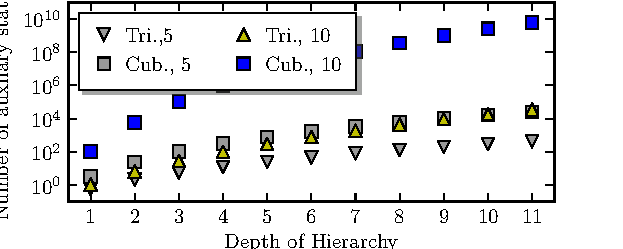
\includegraphics{img/scaling.pdf}
  \caption{Comparison\dots}
  \label{fig:num.scaling}
\end{figure}

% TODO Mention manual cutoff????

%%%%%%%%%%%%%%%%%%%%%%%%%%%%%%%%%%%%%%%%%%%%%%%%%%%%%%%%%%%%%%%%%%%%%%%%%%%%%%%
\section{Correlation Function Expansion}
\label{sec:num.expansion}
% * pade spectrum decomposition
% * also mention other (Matsubara e.g.)
% * uniqueness? Theoretically yes, in practices doesnt matter!
% * Plot for Ohmic spectral density (where do these appear?)
% * Show highly structured density, approximation!
%
% TODO Expansion of general spectral density; not unique!
%      Cool to use antisymmetric lorentzians
% TODO Discussion J(0) = 0 physical necessary, linear (ohmic) decrease, etc.

%%%%%%%%%%%%%%%%%%%%%%%%%%%%%%%%%%%%%%%%%%%%%%%%%%%%%%%%%%%%%%%%%%%%%%%%%%%%%%%

Applicability of our hierarchical equations of motion to any physically interesting system depends predominantly on the ability to express the relevant bath correlation function
\begin{equation}
  \alpha(t) = \int_0^\infty J(\omega) \left( \coth \frac{\beta \omega}{2} \cos \omega(t-s) - \ii\sin \omega(t-s) \right) \mathrm{d}s
  \label{eq:num.alpha_thermal}
\end{equation}
as a sum of exponentials like~\ref{eq:num.exp_bcf}.
Such exponential functions arise as Fourier transforms of a Lorentzian spectral density
\begin{equation}
  J(\omega) = \frac{1}{\pi} \frac{\gamma}{(\omega - \Omega)^2 + \gamma^2}.
  \label{eq:num.lorentzian}
\end{equation}
Hence they can be obtained from \autoref{eq:num.alpha_thermal} in the zero-temperature limit provided we extend the integral domain to include arbitrary negative frequencies as well.
% TODO Keep figure?
This unphysical assumption is a good approximation to the exact case without negative frequencies only for certain parameters as \autoref{fig:num.lorentzian} shows:
For $\gamma\ll\Omega$ the Lorentzian density $J$ is concentrated mostly on the positive semi-axis and the negative frequency contribution to \autoref{eq:num.alpha_thermal} can be neglected.
\begin{figure}
  \centering
  \includegraphics{img/lorentzian}
  \caption{Lorentzian spectral densities (see \autoref{eq:num.lorentzian} for notation).}
  % TODO More caption?
  \label{fig:num.lorentzian}
\end{figure}

A more systematic way to obtain the desired bath correlation function in the case $T > 0$ was proposed by Meier and Tannor \cite{MeTa99_non_markovian}.
They employ anti-symmetrized Lorentzian distributions $\tilde J(\omega) := J(\omega) - J(-\omega)$ to include the negative frequencies without any approximation.
% TODO "Indeed, since" good idea?; Check grammer in general!
Indeed, since $\tilde J$, $\coth$, and $\sin$ are anti-symmetric and $\cos$ is symmetric with respect to reflection at the origin we have
\begin{equation*}
  \int_0^\infty \tilde J(\omega) (\dots) \mathrm{d}\omega = \frac{1}{2}\int_{-\infty}^\infty \tilde J(\omega) (\dots) \mathrm{d}\omega.
\end{equation*}
Of course the same holds true for any anti-symmetric spectral density.
% TODO Mhhh...
However, the bath correlation function does not have the form necessary due to the additional $\coth$ for $T > 0$.
This can only be accomplished approximately by expanding the latter and evaluating \autoref{eq:num.alpha_thermal} using the residue theorem.
We focus on the real part of \autoref{eq:num.alpha_thermal} given by
\begin{equation}
  a(t) = \frac{1}{2} \int_{-\infty}^\infty J(\omega) \coth \frac{\beta\omega}{2} \cos \omega t
  = \frac{1}{2} \int_{-\infty}^\infty J(\omega) \coth \frac{\beta\omega}{2} \exp[ii \omega t],
  \label{eq:num.alpha_thermal_re}
\end{equation}
since it encodes all thermal effects.
Calculating the corresponding imaginary part is straightforward.


%%%%%%%%%%%%%%%%%%%%%%%%%%%%%%%%%%%%%%%%%%%%%%%%%%%%%%%%%%%%%%%%%%%%%%%%%%%%%%%
\subsection{Matsubara Spectrum Decomposition}
\label{sub:num.expansion.matsubara}

A commonly used expansion scheme for the hyperbolic cotangens is the Matsubara spectrum decomposition \cite{Ma00_many_particle}
\begin{equation}
  \coth\left(\frac{\beta \omega}{2}\right) = \frac{2}{\beta} \sum_{n=-\infty}^\infty \frac{1}{\ii\omega_n - \omega},
  \label{eq:num.matsubara_expansion}
\end{equation}
with the Matsubara frequencies $\omega_n = 2\pi n / \beta$.
A short proof and remarks on the convergence of the series above is given in \autoref{sec:coth.matsubara}.
Let us parametrize the anti-symmetrized Lorentzian by
\begin{equation}
  \tilde J(\omega) = \frac{P \omega}{((\omega - \Omega)^2 + \gamma^2) ((\omega + \Omega)^2 + \gamma^2)}
  \label{eq:num.anti_lorentz}
\end{equation}
% TODO Discussion general features
Leaving aside the degenerate case $\gamma = 0$ there are four simple poles of $\tilde J$ given by $\omega = \ii(\pm\Omega \pm\ii\gamma)$.
The symmetry with respect to complex conjugation is due to $\tilde J(\omega)$ being real for $\omega\in\Reals$ whereas point symmetry with respect to the origin carries over from $\tilde J$.
As the singularities of $\tilde J$ and $\coth$ are distinct and do not posses an accumulation point the integral~\ref{eq:num.alpha_thermal_re} can be expressed a sum over individual poles
\begin{equation}
  a(t) = \sum_{\omega = \pm\Omega + \ii\gamma} \Res J(\omega) \coth \frac{\beta \omega}{2} \exp[\ii\omega t]
  + \sum_{\omega_n > 0} \Res \coth \frac{\beta\cdot}{2}(\ii\omega_n) J(\ii\omega_n) \exp[-\omega_n t]
  \label{eq:num.sum_over_poles}
\end{equation}
% TODO Better; J(0) = 0
For $t>0$ we close the integration contour in the upper complex half-plane; hence only poles with non-negative imaginary part need to be included.
Therefore the factor $\exp(-\omega_n t)$ goes to zero as $n\to\infty$ and we can safely truncate the sum at some finite $n_0$.
% TODO Elaborate
This leads exactly to the desired sum-of-exponentials form for the bath correlation function with in general complex parameters; we will discuss the connected problems in\dots\\

% Pros: Simple!!!!
% Cons: Slow convergence

\begin{figure}
  % TODO This picture tells absolutely nothing!
  \centering
  \includegraphics{img/expansions}
  \caption{Comparisson\dots}
  \label{fig:num.expansion}
\end{figure}

%%%%%%%%%%%%%%%%%%%%%%%%%%%%%%%%%%%%%%%%%%%%%%%%%%%%%%%%%%%%%%%%%%%%%%%%%%%%%%%
\subsection{Padé Spectrum Decomposition}
\label{sub:num.expansion.pade}

Although the Matsubara spectrum decomposition provides the desired form for the bath correlation function it is worthwhile to consider alternative schemes---especially since the computational effort of our hierarchical equations of motion depends crucially on the numbers of exponential modes under consideration.
Only recently Hu et al.\ proposed an expansion based on the Padé approximant \cite{HuXuYa10_pade,Hu11_pade}, which is vastly superior to the Matsubara expansion in terms of convergence speed.
% TODO Really?
For further details on the theory of Padé approximants we refer to the book by Baker and Graves-Morris \cite{BaGr96_pade}.

To start off we recall that the hyperbolic cotangens has a simple pole at $z=0$ with $\Res\coth(0) = 1$; therefore we have the convergent Taylor series
\begin{equation}
  f(z) := \coth z - \frac{1}{z} = \lim_{N\to\infty} z \sum_{k=0}^{2N-1} a_k z^{2k} = \lim_{N\to\infty} z \, f_{2N-1}(z)
  \label{eq:num.coth_expansion}
\end{equation}
where we use that $\coth$ as well as $z \mapsto 1/z$ are anti-symmetric function; consequently all even terms in the Taylor series vanish.
By definition of the coefficients $a_k$ we have $f(z) - z \, f_{2N-1}(z) = \mathcal{O}(z^{4N + 1})$ for $\abs{z} < \pi$.
In fact the radius of convergence cannot be increased any further since there are additional singularities of $f$ at $z = \pm\ii\pi$ and the approximating functions $f_N$ are analytical.

% TODO Elimniate the
The main idea in using a Padé approximant is to incorporate these poles into the approximating functions.
The simplest choice is the class of rational functions, that is functions of the form $f_{M,N}(z) = P_M(z) / Q_N(z)$ with polynomials $P_M$ and $Q_N$ of degree less than $M$ and $N$ respectively.
We refer to these as $[M,N]$-approximants.
% TODO Better word than treatment
% TODO Better reason?
In order to simplify the following treatment we only consider approximants of class $[N-1, N]$, which have proven to be especially suitable for Bose-Einstein and Fermi-Dirac distribution function \cite{Hu11_pade}.
Let us also introduce the shorthand notation $x = z^2$.
In order to replace $f_N$ in \autoref{eq:num.coth_expansion} with a $[N-1,N]$ Padé approximant $f_{N-1,N}$, the latter needs to fulfill the interpolation condition
\begin{equation*}
  f_{2N-1}(x) = \sum_k^{2N-1} a_k x^k = \frac{P_{N-1}(x)}{Q_N(x)} + \mathcal{O}(x^{2N})
\end{equation*}
by the usual abuse of notation $f_{2N-1}(z) = f_{2N-1}(x)$.
Unless $Q_N(0) = 0$ this is equivalent to $Q_N(x)f_{2N-1}(x) = P_{N-1}(x) + \mathcal{O}(x^{2N})$, which always has a unique solution as shown by comparing coefficients on both sides.
Using the Padé approximant we can rewrite \autoref{eq:num.coth_expansion} as
\begin{equation}
  \coth(z) = \frac{1}{z} + z \frac{P_{N-1}(z^2)}{Q_N(z^2)} + \mathcal{O}(z^{4N+1})
  \label{eq:num.coth_pade}
\end{equation}

Although $P_{N-1}$ and $Q_N$ are of degree $N-1$ and $N$ respectively there are only $2N$ free parameters because both are only fixed up to a common prefactor.
% TODO Really
Therefore $f_{N-1,N}$ and $f_{2N-1}$ have the same number of coefficients to be determined; details on the numerical implementation can be found in\dots

% TODO CHECK
It is quite remarkable that the Padé approximant not only converges on larger subset of $\Complex$ than the power series in general, but also provides a superior sum-over-poles decomposition compared to the Matsubara expansion \autoref{eq:num.matsubara_expansion}.
It turns out that the roots of $Q_N(x)$ are mutually distinct and negative \cite{HuXuYa10_pade}; therefore we denote them by $\xi_i^2$ ($i=1,\dots,N$).
Replacing the analytic approximant $f_N$ in \autoref{eq:num.coth_expansion} by $f_{N-1,N}$ and expanding the latter in terms of partial fractions gives
\begin{equation}
  \coth\left( \frac{\beta\omega}{2} \right) = \frac{2}{\beta\omega} + \frac{2}{\beta} \sum_{j=1}^N \left( \frac{\eta_j}{\omega + \ii\xi_j} + \frac{\eta_j}{\omega - \ii\xi_j} \right) + \mathcal{O}(\omega^{4N+1})
  \label{eq:num.pade_expansion}
\end{equation}
which agrees with \autoref{eq:num.matsubara_expansion} for $N\to\infty$.
% TODO Correct wording?
It is only for a finite number of summands that the Padé expansion comes to fruition.
% TODO Same notation as above!?
As an example take $N=5$, then we find
\begin{align*}
  \left( \frac{\beta \xi_j}{2\pi j} \right)_j &= (1.00, 1.00, 1.01, 1.18, 2.69) \\
  \left( \frac{\beta\eta_j}{2} \right)_j &= (1.00, 1.00, 1.11, 2.80, 26.59),
\end{align*}
% TODO Too much that
showing a noticeable different behavior than the Matsubara poles and residues given by $\beta \xi_j/2\pi j = 1$ and $\beta \eta_j/2 = 1$ respectively.
Also recall from \autoref{eq:num.sum_over_poles} that the suppressing term for the sum over poles is given by $\exp^{-\xi_j t}$; hence the super-linear growth of the Padé poles ensure that less summands and thus less exponential modes in our hierarchical equations are needed.
In conclusion the Padé spectrum decomposition~\ref{eq:num.pade_expansion} can be interpreted as an optimally corrected truncated Matsubara expansion, where neglected terms are included by adjusting the final poles and residues.






%%%%%%%%%%%%%%%%%%%%%%%%%%%%%%%%%%%%%%%%%%%%%%%%%%%%%%%%%%%%%%%%%%%%%%%%%%%%%%%
\section{Spin-Boson Model}
\label{sec:num.spin_boson}
% * short intro
% * Depth-dependence
% * Terminator dependence
% * lin vs nonlin ✔
% * nr. of realizations for different sets of paramters ✔
% * single trajectories ✔
% * divergences for large coupling --> cause bad truncation
%
% TODO Add application citations
% TODO Better convergence criterion than "looks good"
% TODO What about γ=0 convergence? Sample Size?
% TODO ASKWALTER: How many details on numerical parameters
%%%%%%%%%%%%%%%%%%%%%%%%%%%%%%%%%%%%%%%%%%%%%%%%%%%%%%%%%%%%%%%%%%%%%%%%%%%%%%%

The Spin-Boson model is a well known example in the fields of solid state physics and quantum optics for a dissipative system \cite{}.
Despite being comparatively simple and traceable it shows many characteristics like that can be found in more realistic systems as well:\dots
% TODO Add!
Therefore it is well suited to investigate the properties of a general open quantum system and their dependence on the environmental parameters.
It can also be used to approximately describe systems with a continuous degree of freedom confined by a double well potential \cite{Le87_spinboson}.
Examples for the latter are the motion of defects in some crystalline solids or the motion of the magnetic flux trapped in a superconducting qubit \cite{CaLe83_diss_system}.
% FIXME sounds strange
In this section we use it to further investigate our hierarchy and the dependence on numerical parameters like its depth or the number of realizations.

In general the model is given by a two-level system with the free time evolution described by the Hamiltonian
\begin{equation*}
  \Hsys = - \frac{1}{2}\Delta \sigma_x + \frac{1}{2} \epsilon \sigma_z,
\end{equation*}
% FIXME Check all units
coupled linearly to a bath of harmonic oscillators by $L=c \sigma_z$.
Here $\sigma_i$ denotes the Pauli matrices.

%%%%%%%%%%%%%%%%%%%%%%%%%%%%%%%%%%%%%%%%%%%%%%%%%%%%%%%%%%%%%%%%%%%%%%%%%%%%%%%%
\subsection{Sample Size}
\label{sub:num.spin_boson.sample_size}
%
% TODO Perturbative calculation?
% TODO What about γ


\begin{figure}[p]
  \centering
  \includegraphics{img/linvsnonlin_averaged.pdf}
  % TODO Add parameters
  % TODO Better picutres; varying only one parameter?; better comparable
  \caption{%
    Expectation values for the $\sigma_z$-operator calculated using the linear (left) and nonlinear (right) hierarchical equations for two sets of parameters.
    On the top we display a weakly coupled system given by parameters\dots
    In contrast the bottom pictures show a strongly coupled system with\dots
  }
  \label{fig:num.linvsnonlin}
\end{figure}


% TODO Check this whole paragraph
% TODO Fixed Depth!!
Since our hierarchical equations of motion are based upon a stochastic differential equation, it is crucial to assess their reliability in dependence on the sample size.
In this section we emphasize in particular the superiority of the nonlinear version~\ref{eq:num.hierarchy_nonlin} over the linear hierarchy~\ref{eq:num.hierarchy_lin}.
For a systematic investigation we study the Spin-Boson model using two quite distinct sets of parameters, which we refer to as weakly and strongly coupled, although other parameters as the memory time of the bath $\gamma^{-1}$ have to be taken into account as well.
% TODO Want????
The former choice of parameters can even be treated using an improved perturbation scheme \cite{GaHuZh10_qubit,HuZh08_qubit}.
Nevertheless the nonlinear equations of motion constitute a noticeable improvement in convergence speed even in these almost trivial parameter regimes.\\

In \autoref{fig:num.linvsnonlin} we plot the expectation value of the spin-operator in $z$-direction for an initial eigenstate corresponding to the eigenvalue $s_z = +\frac{1}{2}$.
In the case of the weakly coupled system at the top there seems to be almost no difference between the linear version on the left and the nonlinear version on the right.
Nevertheless for very few realizations the latter is still in better agreement with the more accurate results.
Especially for large times the dampening on the right hand side is more pronounced as comparing the graph for a sample size of ten reveals.

When it comes to the strongly coupled parameter set at the bottom the picture changes dramatically:
First notice that the sample size has to be increased by an order of magnitude to obtain a reliable result.
Notwithstanding the linear version does display any visible change for the different sample sizes shown; hence we cannot expect convergence for even larger numbers of realizations.
Even qualitative features as the vanishing of $\qmean{\sigma_z}$ for $t \to \infty$ cannot be reproduced in this scheme.
It is only for very small times that both sides agree up to a certain extent.
In contrast the nonlinear version improves steadily with growing sample size and provides a good approximation with only minor fluctuations already at 1000 trajectories. \\
% TODO Rough picture correct for N=100

\begin{figure}[t]
  \centering
  \includegraphics{img/normcomp.pdf}
  % FIXME Caption
  \caption{%
    Contributions of single trajectories to the reduced density operator for the linear equations.
    Left: weakly; right: strongly
    For definition see \autoref{eq:num.contribution}\dots
    Parameters are the same as in \autoref{fig:num.linvsnonlin}
    Dotted line = nonlinear.
  }
  \label{fig:num.normcomp}
\end{figure}

% FIXME Two times "To ..."
To understand this behavior recall that we have introduced the nonlinear equations of motion in order to achieve an average over single contributions of the same order of magnitude.
As already mentioned in \autoref{sec:nmqsd.nonlin_nmsse} individual trajectories of the linear version violate this requirement in general.
To get a better assessment of different contributions over time we have to rescale the norm as follows:
First we calculate the reduced density operator $\rho_t$ by the usual Monte-Carlo average
\begin{equation}
  \rho_t = \sum_{n=1}^N \ket{\psi_t(\ZZ_n)} \bra{\psi_t(\ZZ_n)}
  \label{eq:num.monte_carlo_avg}
\end{equation}
over a large number of noise process realizations $\ZZ_n$.
Afterwards we obtain a genuine, normalized density matrix by rescaling with $(\Tr{} \rho_t)^{-1}$.
Therefore we can assess the contribution of a single trajectory $\psi_t(\ZZ_n)$ to \autoref{eq:num.monte_carlo_avg} by $\lfloor \psi_t(\ZZ_n) \rfloor / N$ with
\begin{equation}
  \lfloor \psi_t(\ZZ_n) \rfloor = \sqrt{%
    \frac{\sp{\psi_t(\ZZ_n)}{\psi_t(\ZZ_n)}}{\Tr{} \rho_t}.
  }
  \label{eq:num.contribution}
\end{equation}
Since the states in \autoref{eq:num.monte_carlo_avg} are normalized for the nonlinear equation, we have for its realizations $\lfloor\psi_t(\ZZ_n)\rfloor = 1$.

We display the contribution using the linear version in \autoref{eq:num.normcomp}; clearly we do not obtain a constant contribution for both sets of parameters.
But for the weakly coupled system on the left all trajectories remain roughly the same order of magnitude.
In contrast the contributions on the right hand side belonging to the strongly coupled system all vanish for large $t$, but also show pronounced peaks for a few trajectories.

% FIXME Conclusion
%  * small times ok
%  * additional expense for nonlinear always worth!
In conclusion\dots


%%%%%%%%%%%%%%%%%%%%%%%%%%%%%%%%%%%%%%%%%%%%%%%%%%%%%%%%%%%%%%%%%%%%%%%%%%%%%%%%
\subsection{Hierarchy Depth and Cutoff}
\label{sub:num.spin_boson.depth}

Apart from the sample size there is an even more significant factor limiting the applicability of our hierarchical equations of motion:
As seen from \autoref{fig:num.scaling} the number of auxiliary states required---and with it the computational expense---grows faster then linear with the truncation depth.
Before investigating the latter more thoroughly we demonstrate the effectiveness of using an appropriate terminator instead of just truncating the hierarchy.
For that matter the Spin-Boson model is well suited since contrary to the Dissipative two-level system presented in \autoref{sec:nmqsd.two_level} it does not terminate at any finite order.




\chapter{Application}
\label{chap:app}
% * why?
% * current results/techniques
% transfer of electronic excitation
% preparation: external lase pulse resonant to S_0 -> S_1 transition
% transfer by Coulomb interaction
% state made up by excited electron and a hole (unoccupied electron state in the highest occupied molecule orbital)
% when both are localized at the same molecule: Frenkel exciton
% Examples: molecular crystals of armoatic compounds and rare gases in the solid phase, dye aggregats
% HERE: energy transfer in light harvesting photosyntetic antenna systems
% coherent and incoherent (FÖRSTER) transfer posible
% Time scales (p. 365) ?
%%%%%%%%%%%%%%%%%%%%%%%%%%%%%%%%%%%%%%%%%%%%%%%%%%%%%%%%%%%%%%%%%%%%%%%%%%%%%%%%

% * Growing interest, application, ...
% * to show its working apply our method to energy transfer and absorption spectra of molecular aggregat
% * DEF. Molecular aggregat: assemblies of monomers (molecules, atoms, ...), where monomers largely keep individual properties
%     * interaction leads to collevcitve phenomena
%     * for sake of clarity: monomer = molecule in our notation

%%%%%%%%%%%%%%%%%%%%%%%%%%%%%%%%%%%%%%%%%%%%%%%%%%%%%%%%%%%%%%%%%%%%%%%%%%%%%%%%
\section{Basic Model}
\label{sec:app.model}
% * assumptions
% * Frenkel excitons
%
% FIXME Too many subsections?
% TODO Experimental setup, necessary for app.model.exciton
%%%%%%%%%%%%%%%%%%%%%%%%%%%%%%%%%%%%%%%%%%%%%%%%%%%%%%%%%%%%%%%%%%%%%%%%%%%%%%%%


%%%%%%%%%%%%%%%%%%%%%%%%%%%%%%%%%%%%%%%%%%%%%%%%%%%%%%%%%%%%%%%%%%%%%%%%%%%%%%%%
\subsection{The Aggregat Hamiltonian}
\label{sub:app.model.hamiltonian}

% GENERAL MOLECULE
% ---------------
% * molecular Hamiltonian, Born Oppenheimer approx (large difference in mass)
%     => seperation of time scales,
% * split into electronic and vibrational degrees of freedom
% * in aggregat further vibrational degrees of freedom: inter- and intramolecular as well as solvent
%
% FIXME Rename V_mn since we use it below for matrix elements

In the follwing chapter we treat molecular aggregats with a size in the order of magnitude from a few up to a hundred molecules.
Let us consider the latter composed of electrons and point-like nuclei quantum mechanically described by canonical-conjugated pairs of operators $(p_j, q_j)$ and $(P_j, Q_j)$ respectively.
The corresponding Hamiltonian is given by
\begin{equation}
  \opH{mol} = \opT{el} + \opT{nuc} + \opV{el-el} + \opV{nuc-nuc} + \opV{el-nuc}
  \label{eq:app.mol_hamil}
\end{equation}
% TODO More?
with the kinetic energies $T$ and appropriate Coulomb interactions $V$.
% TODO Really?
We drop possible contributions from internal spin degrees of freedom since they induce only negligible corrections for the systems under consideration.

The vast difference in masses of electrons and nuclei allows us to separate the dynamics of both into two individual parts using the Born-Oppenheimer approximation:
As electrons move on a much faster time scale they can respond to any changes in the nuclear arrangement almost instantaneously.
This amounts to including the motion of nuclei mediated by the Coulomb potential $\opV{el-nuc}$ only adiabatically when calculating the electron dynamics from \autoref{eq:app.mol_hamil}.
% TODO Is this clear and to the point?
Therefor we can reorganize the summands in \autoref{eq:app.mol_hamil} more appropriately to
\begin{equation}
  \opH{mol} = \opH{el}(\QQ) + \opT{nuc} + \opV{nuc-nuc},
  \label{eq:app.mol_hamil_bo}
\end{equation}
where the notation $\opH{el} = \opT{el} + \opV{el-el} + \opV{el-nuc}(\QQ)$ indicates that we regard the electronic Hamiltonian to depend only parametrically on the nuclear coordinates $\QQ$.
% FIXME Notice??
For the processes under consideration only the valence electrons need to be taken into account explicitly; others are included to the nucleon-part without further notice.


% FIXME In all possible combinations?
The same reasoning applies to the complete Hamiltonian of the aggregat, which besides contributions of the form~\ref{eq:app.mol_hamil} for each individual molecule contains intermolecular interactions between electrons and nuclei in all possible combinations.
Therefore it can rephrased similarly to \autoref{eq:app.mol_hamil_bo}
\begin{equation}
  \opH{agg} = \opH{el}(\QQ) + \opT{vib} + \opV{vib-vib},
  \label{eq:app.agg_hamil}
\end{equation}
Here we use the more general notion of vibrational degrees of freedom, which not only comprises the intra- and intermolecular nuclear coordinates, but also possible environmental degrees of freedom not belonging to the aggregat.
These appear for example when studying molecular compounds immersed in a liquid solvent.

% ELECTRONIC PART
% ---------------
% * Holstein model
% * no exchange interaction due to seperation of molecules, no overlap (tight binding)
%     => anti-symmetrization in Hartree anatz non necessary; product basis
%        =>   H_el = Σ_ma ε_ma |φ_ma><φ_ma|  +  ½ Σ ...

The Born-Oppenheimer approximation allows us to analyse the electronic separately from the vibrational part of \autoref{eq:app.agg_hamil} for a fixed coordinate vector $\QQ$.
We split up the former into contributions for each individual electron
\begin{equation*}
  \opH{el} = \sum_m H_m^\mathrm{(el)} + \frac{1}{2} \sum_{m,n} U_{mn}^\mathrm{(el-el)},
\end{equation*}
where $H_m^\mathrm{(el)}$ contains the $m$\th electron's kinetic energy as well as its coupling to the vibrational degrees of freedom and $U_{mn}$ is simply the Coulomb interaction between the $m$\th and $n$\th electron.
The \quotes{free} Hamiltonians $H_m^\mathrm{(el)}$ define distinct electronic states by
\begin{equation*}
  H_m^\mathrm{(el)}(\QQ) \varphi_{ma} (q, \QQ) = \epsilon_{ma}(\QQ) \varphi_{ma} (q, \QQ)
\end{equation*}
for each given environmental configuration $\QQ$.
The index $m$ runs over all electrons under consideration and $a$ is used to label the individual states, which we assume to be ordered by the corresponding energies.
Similar to the Hartree-Fock method we build up an expansion basis for the total electronic state by a product ansatz
\begin{equation}
  \phi_{\vec a}(\qq, \QQ) = \prod_m \varphi_{m, a_m}(q_m, \QQ),
  \label{eq:app.product_states}
\end{equation}
which in general needs to be anti-symmetrized to fulfill the Pauli exclusion principle.

If there is at most one valence electron per molecule we need to take into consideration, which is furthermore tightly bound, then the situation simplifies dramatically:
In this case the spreading of the single-electron states $\ket{\varphi_{ma}} = \ket{m, a}$ is small compared to the distance between two molecules; we can neglect the overlap $\braket{m, a}{n, b}$ for different molecules $m \neq n$.
Consequently \autoref{app.product_states} yields a complete basis for the electronic degrees of freedom.
We also have the following representation for the Hamiltonian~\ref{eq:app.agg_hamil}% FIXME Formula!
\begin{equation}
  \opH{el} = \sum_{m, a} \epsilon_{m, a} \, \ket{m, a}\bra{m, a} + \frac{1}{2}\sum_{m,n,a,b,a',b'} U_{mn}(aa', bb') \, \ket{m,a; n,b}\bra{m,a'; n,b'}
  \label{eq:app.agg_hamil_basis}
\end{equation}
with the matrix elements of the Coulomb interaction\footnote{%
  % TODO Mutual enough?
  This does not include the exchange interaction, since we assume a vanishing mutual overlap for the electrons.
}
\begin{equation*}
  U_{mn}(aa', bb') = \bra{m,a; n,b} U_{mn} \ket{m,a'; n,b'}.
\end{equation*}
% TODO Is this correct?
Note that all terms in \autoref{eq_app.agg_hamil_basis} still depend on vibrational coordinates.
For example the matrix elements $U_{mn}(aa'; bb')$ is influenced by the distance between the $m$\th and $n$\th molecule, while the electronic eigenenergies $\epsilon_{m, a}$ primarily depend on the positions of other electrons belonging to the same molecule.

%%%%%%%%%%%%%%%%%%%%%%%%%%%%%%%%%%%%%%%%%%%%%%%%%%%%%%%%%%%%%%%%%%%%%%%%%%%%%%%%
\subsection{The Exciton Model}
\label{sub:app.model.exciton}
% * beside electronic ground state only first excited singlet state φ_m^g, φ_m^e for each molecule
%     => effective 2 level system
%     * ok if only one S_1 state is initially excited and all first-level energies are same order of magnitude
% * different contributions to interaction term; Heitler-London approximation (p.370)
%     => Interaction term gives only "hopping" contributions (resonant excitation energy transfer)
%     => if we start with single excitation, we remain in the single-excitation Hilbert space
%     => basis vectors |π_n> = |φ_n^e> Π_i≠n |φ_i^g> => single exciton state
%     * need ground state |0> = Π_i |φ_i^g> as well due to dissipation
%     * multi-exciton states for nonlinear stuff
%     * interaction matrix elements can be calculated from center-of-mass coordinate of molecule and Coulomb interaction
%        => more details (dipole approximation, etc.) in spectrum-section
%
% TODO Dipol-Dipol interactoin approximation (p.372)

% TODO Good? Position of footnote?
% FIXME I am too long!!!
In order to describe the experimental setting described in the introduction we do not need to consider the complete electronic Hamiltonian~\ref{eq:app.agg_hamil_basis}:
if only a single valence electron is initially in the lowest excited state $S_1$ above its ground state $S_0$\footnote{%
  Note that $S_0$ describes the lowest energy state of the valence electron with all other electrons of the molecule fixed, not to be confused with the atomic ground states.
}
and if the various transition energies are in the same order of magnitude, then it is sufficient to take only the $S_0$ state $\ket{m, 0}$ as well as the first excited stated $\ket{m, 1}$ for each molecule into account.
% FIXME Is charged induced transition a word?
Under these circumstances the matrix elements $U_{mn}(aa', bb')$ can be classified with respect to a few physical processes such as electrostatic interactions or charge-induced transitions.
But most important is the resonant contribution $U_{mn}(01; 10)$ (and its inversion $U_{mn}(10; 01)$) describing a $S_0 \to S_1$ excitation for the $m$\th electron induced by a  $S_0 \to S_1$ transition at the $n$\th molecule.
In the following we neglect all but the last class of processes, which is frequently called Heitler-London approximation.

Restricting the allowed electronic states to the two lowest energy levels has a remarkable interpretation in terms of quasi-particles:
The product
\begin{equation}
  \ket{m} = \ket{m, 1} \prod_{n \neq m} \ket{n, 0}
  \label{eq:app.exciton_state}
\end{equation}
% TODO What about gorund state?
% FIXME Too much due to, therefore,...
describes an excited electron localized in the vicinity of the $m$\th molecule, which we refer to as an exciton of the electronic system.
Due to the Heitler-London approximation our adiabatic Hamiltonian~\ref{eq:app.agg_hamil_basis} conserves the number of excitons.
Therefore an initial state $\ket{m}$ (or linear combinations thereof) always remains in the one-exciton Hilbert space $\HH^{(1)}$.
% TODO WHY???
The interaction matrix elements
\begin{equation*}
  V_{mn} = V_{nm} = \bra{m, 0; n, 1} U_{mn} \ket{m, 1; n, 0}
\end{equation*}
allow us to express the restriction of $\opH{el}$ to $\HH^{(1)}$ as
\begin{equation*}
  \opH{el}^{(1)}(\QQ) = \sum_m \epsilon_m(\QQ) \ket{m}\bra{m} + \sum_{m,n} V_{mn}(\QQ) \ket{n}\bra{m}.
\end{equation*}
% FIXME Second sentence strange...
For the rest of this section we assume the $V_{mn}$ to be independent of vibrational degrees of freedom; a more general treatment poses no further difficulties.\\

% VIBRATIONAL PART
% ----------------
% * include dynamica

% FIXME Too much "degrees of freedom"
Up to this point we have neglected the dynamical evolution of the vibrational environment, which is essential in a complete description of a molecular aggregat.
% TODO REALLY? WHY?
In common settings for the physical systems under consideration a harmonic approximation is sufficient to obtain a realistic model.
There are two reasons for this:
First of all most proteins disintegrate at temperatures much higher than room temperature; therefore thermal excitation only leads to small energy gains for each vibrational degree of freedom.
The other mechanism for driving the environment is dissipation of the electronic system.
But the latter is small compared to the vast number of vibrational degrees of freedom and energy typically spreads evenly across the environment.
We can thusly assume that all $Q_\lambda$ experience only a small displacement from their equilibrium positions, which we set to $Q_\lambda = 0$.

% TODO More?
As a consequence both $\opV{vib-vib}(\QQ)$ and $\epsilon_m(\QQ)$ can be expanded in a Taylor series neglecting all but the first non-trivial term.
To alleviate notation we further assume that each vibrational degree of freedom only couples to one specific exciton.
This leads to exactly the original model we use to derive the NMSSE: a bath of harmonic oscillators linearly coupled to the electronic system
\begin{align*}
  \opH{agg} =
  \sum_m \epsilon_m(0) \ket{m}\bra{m} + \sum_{m,n} V_{mn} \ket{m}\bra{n} + \sum_{m, \lambda} \omega_{m, \lambda} \adj{A}_{m, \lambda} A_{m, \lambda} \\
  + \sum_{m, \lambda} g_{m, \lambda} \ket{m}\bra{m} \otimes \left( \adj{A}_{m, \lambda} + A_{m, \lambda} \right),
\end{align*}
where $A_{m, \lambda}/\adj{A}_{m, \lambda}$ are ladder operators corresponding to the $\lambda$\th vibrational mode coupling to the $m$\th exciton.


%%%%%%%%%%%%%%%%%%%%%%%%%%%%%%%%%%%%%%%%%%%%%%%%%%%%%%%%%%%%%%%%%%%%%%%%%%%%%%%%
\section{Transfer Dynamics}
\label{sec:app.fmo}
% * FMO
%%%%%%%%%%%%%%%%%%%%%%%%%%%%%%%%%%%%%%%%%%%%%%%%%%%%%%%%%%%%%%%%%%%%%%%%%%%%%%%%

%  * why interesting --> first observed quantum coherence in light harvesting systems
%     => function: connecting large light harvesting antenna;
%        transmit excitation energy to reaction centers
%     * role: avoid local energetic traps; aid efficient trapping of electronic energy by the pigments facing the reaction center \cite{IsFl09_fmo}
%  * important: long-lived electronic quantum coherence
%     => exciton superposition states (formed during fast excitation event) allow the excitation to "reversibly sample all posible paths"
%     => efficient directing the energy transfer to find the most effective sink for the excitation energy \cite{EnCaRe07_photosyn}
%     => efficiency beyond classical sampling-by-hopping
%  * FMO: green sulfur bacteria
%
% * before that: semiclass. hopping (Förster theory)
%

\begin{figure}[t]
  \centering
  \includegraphics[scale=.6]{img/monomer_full600.png}
  % FIXME Better caption
  % FIXME Higher dpi
  \caption{%
    Spatial arrangement of the FMO monomer and numbering of the BChls.
    Here all eight BChls.
    Created using PyMol, based on PDB entry 3ENI \cite{pymol,TrCaBl09_fmo_structure}
  }
  \label{fig:app.monomer_full}
\end{figure}

\begin{figure}[p]
  \centering
  \includegraphics{img/fmo_transfer.pdf}
  % FIXME Caption
  % FIXME Change plot to 2Term fit
  \caption{%
    Exciton transfer of the simplified FMO-monomer with seven BChls using our hierarchical equation of motion up to first~(doted line) and second order~(dashed line).
    We place the initial excitation on both receiving BChls, that is the first~(left) and the sixth molecule~(right).
    For comparison the solid line shows the results of Ishizaki and Fleming~\cite{IsFl09_fmo}, which were obtained in the density-matrix HEOM approach.
  }
  \label{fig:app.fmo_transfer_2}
\end{figure}

\begin{figure}[p]
  \centering
  \begin{subfigure}[b]{0.3\textwidth}
    \includegraphics[width=\textwidth]{img/fmo_transfer_0.png}
    \caption{%
      $t = 0.00 \, \mathrm{fs}$
    }
  \end{subfigure}
  \begin{subfigure}[b]{0.3\textwidth}
    \includegraphics[width=\textwidth]{img/fmo_transfer_1.png}
    \caption{%
      $t = 0.25 \, \mathrm{fs}$
    }
  \end{subfigure}
  \begin{subfigure}[b]{0.3\textwidth}
    \includegraphics[width=\textwidth]{img/fmo_transfer_2.png}
    \caption{%
      $t = 0.50 \, \mathrm{fs}$
    }
  \end{subfigure}
  \vspace{1cm}

  \begin{subfigure}[b]{0.3\textwidth}
    \includegraphics[width=\textwidth]{img/fmo_transfer_3.png}
    \caption{%
      $t = 1.00 \, \mathrm{fs}$
    }
  \end{subfigure}
  \begin{subfigure}[b]{0.3\textwidth}
    \includegraphics[width=\textwidth]{img/fmo_transfer_4.png}
    \caption{%
      $t = 2.00 \, \mathrm{fs}$
    }
  \end{subfigure}

  \caption{%
    Same as \autoref{fig:app.fmo_transfer_2term} with initial excitation on the sixth BChl~(orange).
    Notice how the energy flow is not evenly distributed but shows a pronounced drift towards the energy sink located at the third BChl~(blue).
    For the sake of clarity we do not show the full molecular structure.
  }
\end{figure}

%%%%%%%%%%%%%%%%%%%%%%%%%%%%%%%%%%%%%%%%%%%%%%%%%%%%%%%%%%%%%%%%%%%%%%%%%%%%%%%%
\section{Absorption Spectra}
\label{sec:app.spectra}
% * experimental setup
% * why not so good, but we still use them -> 2D spectroscopy
%%%%%%%%%%%%%%%%%%%%%%%%%%%%%%%%%%%%%%%%%%%%%%%%%%%%%%%%%%%%%%%%%%%%%%%%%%%%%%%%

%%%%%%%%%%%%%%%%%%%%%%%%%%%%%%%%%%%%%%%%%%%%%%%%%%%%%%%%%%%%%%%%%%%%%%%%%%%%%%%%
\subsection{NMSSE for Spectra}
\label{sub:app.spectra.nmsse}
% * why nmsse so good for this?

%%%%%%%%%%%%%%%%%%%%%%%%%%%%%%%%%%%%%%%%%%%%%%%%%%%%%%%%%%%%%%%%%%%%%%%%%%%%%%%%
\subsection{Results}
\label{sub:app.spectra.results}
% * other techniques
% * cool behavior of hierarchies

\chapter{Conclusions}
\label{cha:conclusions}



\appendix
%%%%%%%%%%%%%%%%%%%%%%%%%%%%%%%%%%%%%%%%%%%%%%%%%%%%%%%%%%%%%%%%%%%%%%%%%%%%%%%
%%%%%%%%%%%%%%%%%%%%%%%%%%%%%%%%%%%%%%%%%%%%%%%%%%%%%%%%%%%%%%%%%%%%%%%%%%%%%%%
%\chapter{Mathematical Preliminaries}
%\label{ch:math}
%
%In this chapter we substantiate the claim of \autoref{sub:nmqsd.interpretation.unitary_view}, that the linear non-Markovian Stochastic Schrödinger Equation
%\begin{equation}
%  \partial \psi_t = -\ii h \psi_t + L\ZZ_t \psi_t - \adj{L}\int_0^t \alpha(t-s) \frac{\delta\psi_t}{\delta\ZZ_s} \dd s
%  \label{eq:math.nmsse}
%\end{equation}
%can also be understood as a Schrödinger equation for the unitary time evolution of the system and the environment.
%Our investigation proceeds as follows:
%First we are concerned with the kinematic structure and provide an explicit construction of the underlying bath Hilbert space;
%subsequently we study how the noise process $\ZZ_t$ and the functional derivative in \autoref{eq:math.nmsse} can be realized as operators on this Hilbert space.
%
%Hereinafter we cannot attempt to present a mathematical rigorous treatment of the stochastic differential equation presented above.
%Instead our main goal is to provide a basic understanding how \autoref{eq:math.nmsse} fits into the established framework of Stochastic Analysis and more important how an interpretation in terms of ladder operators is justified.
%In our construction we closely follow the ideas of White Noise Analysis \cite{Hi80_brownian_motion,HiKuPoSt93_white_noise}.
%
%%%%%%%%%%%%%%%%%%%%%%%%%%%%%%%%%%%%%%%%%%%%%%%%%%%%%%%%%%%%%%%%%%%%%%%%%%%%%%%%
%\section{Hilbert Space of \quotes{Time Oscillators}}
%\label{sec:math.hilbert_space}
%%
%%TODO besser erklären, wie verschiede versionen zustande kommen
%%TODO reference
%%TODO ZZ_t explizit nochmal reinschreiben?
%%TODO Abkürzungen? NMSSE? BCF?
%%TODO interpretation von Ω?
%%%%%%%%%%%%%%%%%%%%%%%%%%%%%%%%%%%%%%%%%%%%%%%%%%%%%%%%%%%%%%%%%%%%%%%%%%%%%%%%
%
%Let us first recall some basic terminology from probability theory (see e.g.~\cite{Sc05_mims}):
%A $C$-valued \idef{random variable} $X$ is a measurable map from a measure space $(\Omega, \mathcal{A}, \PM)$ to the measurable space $(C, \mathcal{B})$.
%Here $\Omega$, $C$ denote sets, $\mathcal{A}$, $\mathcal{B}$ are $\sigma$-algebras of $\Omega$ and $C$ respectively, and $\PM$ is a probability measure on $(\Omega, \mathcal{A})$.\footnote{In what follows, we will consider only Borel-$\sigma$-algebras and therefore not mention them any further.}
%Expectation values, variances, etc., may then be expressed as integrals of $X$ with respect to $\PM$.
%
%%TODO Satz fertig
%It is important to mention, that --- versions\dots
%Therefore we may always use the version of $\ZZ_t$ defined in the microscopical model as
%\begin{equation*}
%  \ZZ_t(\zz) = -\ii \sum_{\lambda=1}^N \cc g_\lambda \cc z_\lambda \exp[\ii \omega_\lambda t]
%\end{equation*}
%with $\Omega=\Complex^N$ and $\PM=\exp[-\abs\zz^2]\dd^Nz$.
%But since this is---strictly speaking---valid only for a finite number $N$ of bath oscillators, we will take a different route:
%Using only the bath correlation function defined by
%\begin{equation}
%  \alpha(t) = \int_\Reals \exp[-\ii\omega t] \, J(\omega)\dd\omega
%  \label{eq:math.def_alpha}
%\end{equation}
%we establish a suitable measure space, which will be used to support our new environmental Hilbert space afterwards.
%Such a unified approach has the advantage of only making reference to the bath correlation function, stressing that it is the only property of the environment relevant within our model.
%Here $J(\omega)\dd\omega$ denotes the \idef{spectral density} formally represented by a positive, bounded measure, that is $J\ge0$ and $\int J(\omega)\dd\omega < \infty$.
%Although the latter condition excludes the important Markov limit $\alpha(t)\propto\delta(t)$ derived from a constant spectral density we can treat it along the same lines.
%
%%TODO Write down conventions for Fourier Transform.
%As a starting point we introduce the probability space $\Omega$ replacing the coherent state labels $(z_1, \dots, z_N)$.
%In what follows the \idef{Schwartz space} $\SchwartzS$ of real valued, infinitely often differtiable functions on $\Reals$ with rapid decrease plays an important role---see \cite[Chap.~7]{Ru91_functional_analysis} for its definition and properties.
%The reason for its importance is found in the following theorem.
%\begin{thm}[Minlos's Theorem, {{\cite[Thm.~1.1]{HiKuPo93_white_noise}}}]
%  \label{thm:math.minlos}
%  Let $\CHF$ be a characteristic functional on $\SchwartzS$, i.e. $\CHF\colon \SchwartzS \rightarrow \Reals$ with the properties
%  \begin{enumerate}[i)]
%    \item $\CHF$ is continous on $\mathcal{S}$,
%    \item $\CHF$ is positive definite,
%    \item $\CHF(0) = 1$.
%  \end{enumerate}
%  Then there exists a unique probability measure $\PM$ on $\dual{\SchwartzS}$ (the dual space of $\SchwartzS$), such that for all $f \in\SchwartzS$
%  \begin{equation}
%    \int_{\dual{\SchwartzS}} \exp[\ii \, \dualp{\xi}{f}] \dd\mu(\xi) = \CHF(f).
%    \label{eq:math.fourier_minlos}
%  \end{equation}
%\end{thm}
%
%Here $\dualp{\xi}{f}$ denotes the dual pairing of $\SchwartzS/\dual{\SchwartzS}$, which can formally be written as $\dualp{\xi}{f} = \int_\Reals \xi(t) f(t) \, \dd t$.
%We also recall that a function $f$ is called \idef{positive definite}, if\dots
%%TODO Insert definition POSTIVE DEFINITE
%In \cite{HiKuPo93_white_noise} they take advantage of this theorem to construct a real valued White Noise processes on $\dual\SchwartzS$ with the choice $\CHF(f) = \exp(-\int_\Reals f(t)^2 \dd t)$.
%This can be rephrased as $\CHF(f)=\exp(-\,\varf(f,f))$ with the \emph{variance functional} $\varf(f,f) =\int f(t)^2 \dd t$.\\
%
%But since we are interested in complex processes with memory we need to generalize these results in two directions.
%Notice how the variance functional from the last paragraph can be understood as Markov limit of the more general form
%\begin{equation}
%  \varf(f,f) = \int_{\Reals^2} \alpha(t-s) f(t) f(s) \dd t \dd s \quad (f \in\SchwartzS).
%  \label{eq:math.def_varfunc}
%\end{equation}
%
%
%
%%It turns out to be crucial for what follows that the variance functional always provides additional structure on our probability space.
%%\begin{lem}
%%  Let $\alpha$ be a correlation function, that is a Fourier transform of a bounded measure. Then
%%  \begin{equation}
%%    \varf(f, g) := \iint \alpha(t - s) \, f(t) \, g(s) \dd t \dd s \quad (f, g \in \SchwartzS)
%%    \label{eq:math.covf_sp}
%%  \end{equation}
%%  defines a real scalar product on $\SchwartzS$.
%%  Additionally $\varf$ is separately continuous in each component with respect to $\SchwartzS$.
%%  \label{lem:math.covf_sp}
%%\end{lem}
%%For the proof we need an important property of the Fourier transform when acted on test functions with rapid decrease.
%%% TODO Fix spaces!
%%% TODO Too much formula, more words!
%%\begin{lem}[{{\cite[Thm.~7.7]{Ru91_functional_analysis}}}]
%%  Let $\SchwartzSC=\SchwartzS+\ii\SchwartzS$ denote the complexified space of test-functions.
%%  Put differently $f \in \SchwartzSC \iff \Re{f}, \Im{f} \in \SchwartzS$.
%%  The Fourier transform is a continuous, linear one-to-one mapping of $\SchwartzSC$ onto $\SchwartzSC$.
%%  \label{lem:math.fourier}
%%\end{lem}
%%% TODO Does this look ok?
%%\begin{proof}[Proof of Lemma~\ref{lem:math.covf_sp}]
%%  Since $\abs{\alpha(t)} \le \int J(\omega)\dd\omega =: A < \infty$, we have for any $f,g\in\SchwartzS$
%%  \begin{equation*}
%%    \abs{\varf(f,g)} \le \iint \abs{\alpha(t-s) f(t) g(s)} \dd s \dd t
%%                     \le A \int\abs{f(t)}\dd t \, \int\abs{g(s)}\dd s
%%                     < \infty,
%%  \end{equation*}
%%  where we used that all test-functions are also integrable.
%%  Continuity also follows from this inequality, since convergence in the $\SchwartzS$-sense implies $L^1$-convergence.
%%
%%  Linearity and symmetry are trivial; therefore we only need to check that $\varf(f,f)=0$ implies $f=0$.
%%  Using Lemma~\ref{lem:math.fourier} we find a $\ift{f}\in\SchwartzSC$ with $\int\exp[-\ii\omega t]\ift{f}(\omega)\dd\omega = f(t)$.
%%  A short calculation then reveals
%%  \begin{align*}
%%    \varf(f,f) & = \iint \alpha(t-s) f(t) f(s) \dd t \dd s = \iint \alpha(t-s) \cc{f(t)} f(s) \dd t \dd s \\
%%               & = \iint  \int\exp[-\ii \Omega (t-s)]J(\Omega)\dd\Omega  \int\exp[\ii\omega t]\cc{\ift{f}(\omega)}\dd\omega  \int\exp[-\ii\omega' s]\ift{f}(\omega') \dd\omega'  \dd s \dd t \\
%%               & = \iiint \left(   \int \exp[-\ii(\Omega - \omega)t] \dd t  \int \exp[\ii(\Omega - \omega')s] \dd s  \right) \cc{\ift{f}(\omega)}\ift{f}(\omega') J(\Omega) \dd\Omega \dd\omega \dd\omega' \\
%%               & \propto \int \abs{\ift{f}(\Omega)}^2 J(\Omega) \dd\Omega.
%%  \end{align*}
%%  Therefore $\varf(f,f)=0$ implies $\ift{f}=0$, leading to the conclusion $f=0$.
%%\end{proof}
%%\begin{rem}
%%  For the Markovian regime the statement holds true as well, since $\varf$ coincides with the $L^2$-scalar product in that case.\\
%%\end{rem}
%
%However, we cannot apply \autoref{thm:math.minlos} directly to $\CHF(f)=\exp[-\, \varf(f,f)]$ because it does not apply to the complexified space $\SchwartzSC$.
%Instead we will follow the strategy in \cite{Hi80_brownian_motion}: first we restrict $\varf$ to $\SchwartzS$, where it does not necessarily have the form \eqref{eq:math.def_covf}.
%
%
%
%We want complex Hilbert space, Minlos only works with real. First define complex one, read of ``real'' sp, complexify again. Define $\alpha$ as FT, Define complex Pre-Hilbert space; define Complexification of $\SchwartzS$
%\begin{lem}
%  $\sp{\cdot}{\cdot}$ is well defined scalar product, continous on $\SchwartzS_\Complex$
%\end{lem}
%Complete $\SchwartzS_\Complex$; Hilbert Space $\mathcal{H}_\Complex$
%\begin{lem}
%  $\mathcal{H}_\Complex$ is seperable
%\end{lem}
%
%Go over to $\SchwartzS$, what is scalar product, use polarisation; show that complexified scalar product gives back old scalar product
%\begin{thm} \label{thm:mp_existence}
%  On $(\dual{\mathcal{S}_\Complex}, \mathcal{B})$ there exists a Gauss Measure $\mu$ such that for $f \in \SchwartzS_\Complex$
%  \begin{equation}
%    \label{eq:mp_fourier_gauss}
%    \int_{\dual{\SchwartzS_\Complex}} \exp{\left(\ii \, \Re(\xi, f)\right)} \dd\mu(\xi) = \exp(-\frac{1}{4} \Vert f \Vert_\mathcal{H})
%  \end{equation}
%\end{thm}
%
%Define $(L^2)$; scalar product; In the language of probability theory we have prop space $(\dual{\SchwartzS_\Complex}, \mathcal{B}, \mu)$. For $f,g \in \SchwartzS$ we have random variables $\cc{(\cdot, f)}$ and $(\cdot, g)$ such that $\E \ldots$. Can be continued to $\mathcal{H}$; later $Z_t := (\cdot, \delta_t)$; Formally
%  \begin{equation*}
%  (\xi, f) = \int \xi(t) f(t) \dd t = \int \int \xi(s) \delta(s-t) \dd s f(t) \dd t = \int (\cdot, \delta_t) f(t) \dd t
%  \end{equation*}
%Therefore $(\cdot, f) = \int Z_t f(t) \dd t$; Formal scalar product; Example Brownian motion,
%
%  \begin{thm} \label{thm:mp_expansion}
%  $(L^2)$ has the following ONB\dots
%  \end{thm}
%Symmetric Fock Space, how to recover microscopical model
%
%
%%%%%%%%%%%%%%%%%%%%%%%%%%%%%%%%%%%%%%%%%%%%%%%%%%%%%%%%%%%%%%%%%%%%%%%%%%%%%%%%
%\section{Noise Creation- and Anhilation Operators}
%\label{sec:math.operators}
%% * prove of Novikov Formula
%%%%%%%%%%%%%%%%%%%%%%%%%%%%%%%%%%%%%%%%%%%%%%%%%%%%%%%%%%%%%%%%%%%%%%%%%%%%%%%%
%
%On all elements with finite expansion, $f \in \mathcal{H}$ define $\op Z_f$; calculate Adjoint, Formal notation, define $\op Z_t$


%%%%%%%%%%%%%%%%%%%%%%%%%%%%%%%%%%%%%%%%%%%%%%%%%%%%%%%%%%%%%%%%%%%%%%%%%%%%%%%
%%%%%%%%%%%%%%%%%%%%%%%%%%%%%%%%%%%%%%%%%%%%%%%%%%%%%%%%%%%%%%%%%%%%%%%%%%%%%%%
\chapter{Analytic Solution of Dissipative Two-level System}
\label{ch:tla}

%%%%%%%%%%%%%%%%%%%%%%%%%%%%%%%%%%%%%%%%%%%%%%%%%%%%%%%%%%%%%%%%%%%%%%%%%%%%%%%
\section{General Solution}
\label{sec:tla.general}
%
% TODO Better title

Here we present in full detail the analytic solution of the dissipative two-level system introduced in \autoref{sec:nmqsd.two_level}.
The relevant NMSSE can always be written in terms of a single process
\begin{equation}
  \partial_t \psi_t = -\ii\frac{\omega}{2}\sigma_z\psi_t + c \sigma_- \ZZ_t \psi_t - c\sigma_+ \int \alpha(t - s) \frac{\delta\psi_t}{\delta \ZZ_s} \dd s.
  \label{eq:tla.nmsse_twolevel}
\end{equation}
As already mentioned we employ an ansatz for the quantum trajectory at most linear in $\ZZ_s$
\begin{equation}
  \psitZ = \psi(t) + \int_0^t \psi_s(t) \ZZ_s \dd s.
  \label{eq:tla.ansatz}
\end{equation}
% TODO Better footnote
Here we already incorporate that $\psitZ$ needs to be independent of $\ZZ_s$ for $s < 0$ and $s>t$ by using a bounded integral domain.\footnote{A consistent treatment of these independence-conditions is more tricky than it seems at first glance, since we are mixing a distributional object $\ZZ_s$ with a discontinuous function $s \mapsto \psi_s(t)$.
  As $\delta \psi_t(\ZZ) / \delta \ZZ_s = 0$ translates to $\psi_s(t) = 0$ the correct integral boundary reads $\int_{0-\varepsilon}^{t+\varepsilon}$ with $\varepsilon > 0$ but arbitrary otherwise.
  \label{fn:tla.boundaries}
}
We use a basis for $\psi_t(\ZZ)$ which renders $\sigma_z$ diagonal and denote the corresponding components by \quotes{+} and \quotes{-}.
The \quotes{+}-component of our NMSSE with the ansatz~\ref{eq:tla.ansatz} reads
\begin{align}
  \dot\psi^+(t) + \psi^+_t(t)\ZZ_t &+ \int_0^t \dot\psi^+_s\ZZ_s \dd s \nonumber\\
  &= -\ii \frac{\omega}{2} \left( \psi^+(t) + \int_0^t \psi^+_s(t)\ZZ_s \dd s \right) - c \int_0^t \alpha(t-s) \psi^-_s(t) \dd s.
  \label{eq:tla.psi_plus}
\end{align}
In order to separate contributions of different order in $\ZZ_s$, we apply the functional derivative $\delta/\delta\ZZ_s$ with arbitrary $s$ to the last equation
\begin{equation}
  \psi^+_t(t) \delta(t - s) + \int_0^t \dot\psi^+_{s'}(t) \delta(s - s') \dd s' = -\ii \frac{\omega}{2} \int_0^t \psi^+_{s'}(t) \delta(s - s') \dd s'.
  \label{eq:tla.psi_plus_deriv}
\end{equation}
Choosing $s \in (0, t)$ leaves us with a simple ordinary differential equation with solution $\psi^+_s(t) = C_s \exp[- \ii \omega t / 2]$.
By further investigating the singular term in \autoref{eq:tla.psi_plus_deriv} we find that $\psi^+_s(s)$ and therefore the constant $C_s$ must vanish.
This amounts formally to integrating~\ref{eq:tla.psi_plus_deriv} over a small interval $(t-\varepsilon, t+\varepsilon)$ with respect to $s$.
In the limit $\varepsilon \to 0$ all terms except the first go to zero.
On the other hand we can isolate all terms independent of $\ZZ_s$ in \autoref{eq:tla.psi_plus} simply by taking the expectation value.
The resulting equation
\begin{equation}
  \dot\psi^+(t) = -\ii \frac{\omega}{2} \psi^+(t)  - c \int_0^t \alpha(t - s) \psi^-_s(t) \dd s
  \label{eq:psi_plus_expect}
\end{equation}
is treated later, once we have an explicit expression for $\psi^-_s(t)$.

The \quotes{-} component of \autoref{eq:tla.nmsse_twolevel} is quite similar to~\ref{eq:tla.psi_plus}
\begin{align}
  \dot\psi^-(t) + \psi^-_t(t)\ZZ_t &+ \int_0^t \dot\psi^-_s(t)\ZZ_s \dd s \nonumber \\
  &= \ii \frac{\omega}{2} \left( \psi^-(t) + \int_0^t \psi^-_s(t)\ZZ_s \right) + c \psi^+(t)\ZZ_t,
  \label{eq:tla.psi_minus}
\end{align}
where we already used that $\psi^+_s(t) = 0$.
The solution
\begin{equation}
  \psi^-(t) = \psi^-(0) \, \exp[\ii \frac{\omega}{2} t]
\end{equation}
can be read off \autoref{eq:tla.psi_minus} directly by comparing all terms independent of $\ZZ_t$.
In the same manner as we derived \autoref{eq:tla.psi_plus_deriv} we can treat all terms proportional to $\ZZ_t$.
Again we find a solution of the form $\psi^-_s(t) = C_s \exp[\ii\omega t / 2]$; the only difference is an additional singular term due to the driving process in \autoref{eq:tla.nmsse_twolevel}.
It gives rise to the boundary condition $\psi^-_t(t) = c \psi^+(t)$.
Together with~\ref{eq:tla.psi_plus_expect} we obtain a closed equation for $\psi^+(t)$
\begin{equation}
  \dot\psi^+(t) = -\ii \frac{\omega}{2} \psi^+(t) - c^2 \int_0^t \alpha(t - s) \exp[\ii \frac{\omega}{2} (t - s)] \psi^+(s) \dd s.
  \label{eq:tla.psi_plus_eq}
\end{equation}
Hence we may replace the original NMSSE~\ref{eq:tla.nmsse_twolevel} by a $\Complex$-valued equation similar in structure.


%%%%%%%%%%%%%%%%%%%%%%%%%%%%%%%%%%%%%%%%%%%%%%%%%%%%%%%%%%%%%%%%%%%%%%%%%%%%%%%
\section{Exponential Correlation Function}
\label{sec:tla.exp}

As \autoref{eq:tla.psi_plus_eq} still contains a memory integral there is no analytic solution in general.
The situation is noticeably simpler for a bath correlation of the form
\begin{equation}
  \alpha(t - s) = \sum_{j=1}^N g_j \, \exp[-\gamma_j \abs{t - s} - \ii \Omega_j (t - s)].
  \label{eq:tla.exp_alpha}
\end{equation}
Since $\psi^+$ only depends on values of $\alpha(t)$ for $t \ge 0$ we can assume $\gamma = 0$ without loss of generality.
Similar to our hierarchical equations of motion elaborated in \autoref{sec:num.sheom} we absorb the problematic terms into auxiliary functions
\begin{equation}
  \phi_j(t) := \int_0^t \alpha_j(t-s) \exp[\ii \frac{\omega}{2}(t-s)] \psi^+(s) \dd s.
  \label{eq:tla.auxiliary}
\end{equation}
This allows us to rewrite \autoref{eq:tla.psi_plus_eq} as a system of $(N+1)$ ordinary differential equations with constant coefficients
\begin{align*}
  \dot\psi^+(t) &= -\ii \frac{\omega}{2} \psi^+(t) - c^2 \sum_{j=1}^N \phi_j(t) \\
  \dot\phi_j(t) &= g_j \psi^+(t) + \ii \left( \frac{\omega}{2} - \Omega \right) \phi_j(t).
\end{align*}
and initial conditions $\phi_j(0) = 0$.
In the special case $N = 1$ the diagonalization can be carried out analytically.
With the shorthand notation $\tilde\Omega = \sqrt{(\omega - \Omega)^2 + 4c^2 g}$ the solution to \autoref{eq:tla.psi_plus_eq} reads
\begin{equation}
  \psi^+(t) = \frac{\psi^+(0)}{2\tilde\Omega} \left( (\omega - \Omega + \tilde\Omega) \, \exp[-\ii \frac{\Omega + \tilde\Omega}{2} t ]  -  (\omega - \Omega - \tilde\Omega) \, \exp[-\ii \frac{\Omega - \tilde\Omega}{2} t ] \right).
  \label{eq:tla.solution}
\end{equation}

%

%%%%%%%%%%%%%%%%%%%%%%%%%%%%%%%%%%%%%%%%%%%%%%%%%%%%%%%%%%%%%%%%%%%%%%%%%%%%%%%
%%%%%%%%%%%%%%%%%%%%%%%%%%%%%%%%%%%%%%%%%%%%%%%%%%%%%%%%%%%%%%%%%%%%%%%%%%%%%%%
\chapter{Expansions of Hyperbolic Cotangens}
\label{cha:coth}
%
% * punktierte Umgebung = punctured

Before presenting the two expansion schemes for the hyperbolic cotangens function mentioned in \autoref{sec:num.expansion} we need to introduce a few ideas from complex analysis.
For more details and proofs we refer to the book of Rudin \cite{Ru87_analysis}.

% TODO Is this already enough citation?
First recall that a function $f$ with an isolated singularity $a\in\Complex$ can always be expanded in a Laurent series around $a$
\begin{equation}
  f(z) = \sum_{j=0}^\infty a_j (z - a)^j + \sum_{j=1}^\infty \frac{a_{-j}}{(z-a)^j} \qquad (0 < \abs{z-a} < \varepsilon).
  \label{eq:coth.laurent}
\end{equation}
% TODO Mention punctured environment
The first sum is called \idef{analytical part} while the second one is called \idef{principal part}.
Clearly if $a$ is a removable singularity, that is the principal part vanishes, we can continue $f$ to a function analytical for all $z$ with $\abs{z-a} < \varepsilon$.
A complex function $f$ is said to be \idef{meromorphic} in an open set $\Omega\subset\Complex$ if it is analytical on $\Omega$ except a set $A \subset\Omega$ of isolated points, which are poles for $f$.
%Roughly speaking meromorphic functions are analytical leaving out some isolated poles; this reading is further substantiated by the following theorem.
%\begin{thm}[Mittag-Leffler, {{\cite[13.10]{Ru87_analysis}}}]
%  Suppose $\Omega$ is an open set in the complex plane, $A \subset \Omega$ has no limit points in $\Omega$, and to each $a \in A$ there is a polynomial of finite order $P_a(z)$ in $1/(z-a)$, that is
%  \begin{equation*}
%    P_a(z) = \sum_{j=1}^{o(a)} \frac{c_{j,a}}{(z-a)^j}.
%  \end{equation*}
%  Then there exists a meromorphic function $f$ in $\Omega$, whose principle part at each $a \in A$ is $P_a$ and which has no further singularities in $\Omega$.
%  \label{thm:coth.mittag_leffler}
%\end{thm}
%Clearly the choice of such a $f$ is not unique as we can always add a function analytical in $\Omega$ to $f$.
%On the other hand this exhausts all possibilities: if $f$ and $f'$ both satisfy the conditions mentioned above then they have identical isolated singularities given by the elements of $A$.
%The same applies to their difference $g = f - f'$; but since all principle parts for $f$ and $f'$ at each $a \in A$ match, we can continue $g$ to an analytical function on $\Omega$.

%%%%%%%%%%%%%%%%%%%%%%%%%%%%%%%%%%%%%%%%%%%%%%%%%%%%%%%%%%%%%%%%%%%%%%%%%%%%%%%
\section{Matsubara Expansion}
\label{sec:coth.matsubara}

In \autoref{sec:num.expansion} we use the expansion of the hyperbolic cotangens in terms of Matsubara frequencies \cite{Ma00_many_particle}
\begin{equation}
  \omega_n = \frac{2\pi n}{\beta} \qquad (n \in \Integers).
  \label{eq:coth.matsubara_freq}
\end{equation}
It provides a sum over poles representation, namely
\begin{equation}
  % TODO Check
  \coth\left(\frac{\beta z}{2}\right) = \frac{2}{\beta} \sum_{n=-\infty}^\infty \frac{1}{\ii\omega_n - z},
  \label{eq:coth.matsubara_expansion}
\end{equation}
with singularities evenly distributed along the imaginary axis.

In order to proof \autoref{eq:coth.matsubara_expansion} notice that $\ii\omega_n$ are exactly the isolated singularities of $z \mapsto \coth(\beta z / 2)$.
Indeed, using the representation
\begin{equation}
  f(z) := \coth\left(\frac{\beta z}{2}\right) = \frac{1 + \exp[-\beta z]}{1 - \exp[-\beta z]}
  \label{eq:coth.representation}
\end{equation}
we see that the numerator as well as the denominator are analytical for all $z \in \Complex$, but the latter vanishes for $z = \ii \omega_n$.
% TODO Elaborate?
A short calculation reveals that these $z$ are simple poles with $\operatorname{Res}f(\ii\omega_n) = 2/\beta$.

Let us now define $g$ by the right hand side of \autoref{eq:coth.matsubara_expansion}; in order to enforce convergence of the infinite series, we need to take the symmetric limit
\begin{equation}
  g(z) = \frac{2}{\beta} \, \lim_{N\to\infty} \sum_{n=-N}^{N} \frac{1}{\ii\omega_n - z} = - \frac{2}{\beta} \, \left( \sum_{n=0}^\infty \frac{2z}{\omega_n^2 + z^2} + \frac{1}{z} \right)
  \label{eq:coth.series}
\end{equation}
where we used $\omega_{-n} = -\omega_n$ in the second step.
Since $\omega\propto n$ the infinite series for $g$ in \autoref{eq:coth.series} converges absolutely unless $z = \ii\omega_n$ and defines a meromorphic function with the same poles and principal parts as $f$.
This leads to the conclusion that $h := f - g$ can be continued to an analytical function on the entire complex plane.
We now show that $h$ is bounded on $\Complex$ and therefore a constant function by Liouville's Theorem.
% TODO Fill in!
Expanding both $f$ and $g$ in a Laurent series about 0 allows us to calculate $f() = g() = $ as % lies within the convergence disk of both series.
In conclusion we find $h = 0$, or put differently $f = g$---the Matsubara expansion~\ref{eq:coth.matsubara_expansion} is valid on the entire complex plane.

% TODO Boundness of h!!
%
% Idea: Show f and g are bounded for Re z --> infinty; enough since periodic


\bibliographystyle{alpha}
%\bibliographystyle{plain}
\bibliography{references}

\newpage
\section*{\centering{Danksagung}}\bigskip
\thispagestyle{empty}

An erster Stelle möchte ich mich natürlich ganz herzlich bei Herr Prof. Strunz für die Betreuung während der Diplomarbeit bedanken.
Sie haben es mir durch die Freiheit bei der Aufgabenstellung ermöglicht, den Verlauf dieser Arbeit größtenteils selber zu bestimmen.
Außerdem haben Sie mich in zahlreichen Diskussionen immer wieder auf den richtigen Weg zurückgebracht.
Weiterhin möchte ich bei Herr Dr. Großmann dafür bedanken, dass er sich als Zweitgutachter zur Verfügung gestellt hat.\\

Alexander Eisfeld möchte ich für die vielen Gespräche, Korrekturen und Hinweise danken, die maßgeblich zum Entstehen dieser Arbeit beigetragen haben---auch wenn mein erster Entwurf allen deinen Veröffentlichungen widersprach.
Gerhard Ritschel möchte ich für seine Hilfe bei vielen Details der Rechnungen und für seine Unterstützung bei allem was mit Temperatur zu tun hat bedanken.\\

Natürlich wäre diese Danksagung nicht vollständig ohne eine Erwähnung der ganzen TQO-Arbeitsgruppe.
Insbesondere möchte ich mich bei Franziska Peter bedanken, auch wenn ich nicht sagen darf wofür.
Lena Simon möchte ich für das Korrekturlesen in sprichwörtlich letzter Minute danken.
Bei Richard Hartmann möchte ich mich für die Diskussionen und Erkenntnisse zum Thema dieser Arbeit bedanken, auch wenn ich glaube dass $\gamma \neq 0$ gelten sollte.\\

Bei meinen Eltern möchte ich herzlichst für die tatkräftige Unterstützung während der Studienzeit bedanken.





% Alex
% Gerhard
%
% Franzi, Lena
% Richard
% Rest der Arbeitsgruppe
%

\newpage
\selectlanguage{ngerman}
\thispagestyle{empty}
\section*{\centering{Erklärung}}\bigskip

Hiermit versichere ich, dass ich die vorliegende Arbeit ohne unzulässige Hilfe Dritter und ohne Benutzung anderer als der angegebenen Hilfsmittel angefertigt habe. Die aus fremden Quellen direkt oder indirekt übernommenen Gedanken sind als solche kenntlich gemacht. Die Arbeit wurde bisher weder im Inland noch im Ausland in gleicher oder ähnlicher Form einer anderen Prüfungsbehörde vorgelegt.\\[2.3cm]
Daniel Süß\\
Dresden, \today
\end{document}
